% !TeX root = digital-platform-api-economy.tex
% !TeX encoding = UTF-8
\chapter{Monetisasi API dan Metrik Platform}
\label{ch:ch12}

% Kolom rata kiri untuk tabel bab ini: G selebar sisa tabel, H selebar yang ditentukan.
\newcolumntype{G}{>{\raggedright\arraybackslash}X}
\newcolumntype{H}[1]{>{\raggedright\arraybackslash}p{#1}}
\lstdefinestyle{ch12python}{language=Python, basicstyle=\ttfamily\scriptsize, keywordstyle=\color{blue}\bfseries,
  commentstyle=\color{gray}\itshape, stringstyle=\color{red}, showstringspaces=false, breaklines=true, frame=lines,
  captionpos=b, xleftmargin=8pt, columns=fullflexible, keepspaces=true, tabsize=2}

\section*{Tujuan Pembelajaran}
\begin{itemize}
  \item Membedakan nilai API langsung dan tidak langsung beserta contoh penerapannya.
  \item Memilih model harga API yang sesuai dengan strategi platform dan sisi pasar.
  \item Menyusun pohon metrik yang menghubungkan aktivitas API dengan tujuan bisnis.
\end{itemize}

\section{Pendahuluan}

\textit{Application Programming Interface} (API) internal Medikara tidak menjual panggilan, tetapi dapat mengurangi telepon
dan pekerjaan ulang. API mitra juga belum tentu perlu diberi harga per permintaan. Bab 2 mengusulkan klinik mitra membayar
Rp3 juta per bulan, atau Rp1,44 miliar per tahun untuk 40 klinik. Bab 4 menyediakan Rp180 juta per tahun agar API klaim
dikelola sebagai produk, walaupun API itu tidak dijual. Bab 11 mencatat 12 klinik yang berhenti berarti kehilangan Rp432
juta per tahun. Pertanyaan kemudian muncul: siapa menerima manfaat, siapa membayar, unit apa yang ditagih, dan angka apa
yang membuktikan nilainya?

Pembedaan nilai menjawab pertanyaan pertama. Model harga dan struktur pasar menjawab pertanyaan kedua dan ketiga. Titik
impas dan pohon metrik menjawab pertanyaan terakhir. Bab ini memakai angka dari bab sebelumnya: 20 sambungan aktif, Rp45
juta per antarmuka, tarif Rp60.000 per jam, biaya lapisan bersama Rp300 juta per tahun, dan kuota 300 panggilan per hari
per klinik. Angka tambahan yang diawali kata ``Misalkan'' adalah asumsi latihan. Kesimpulan untuk organisasi nyata harus
diuji dengan wawancara, dokumen, dan pengukuran yang berizin. \textit{Business case} dibahas rinci di IT40513, sedangkan
pelaporan \textit{Key Performance Indicator} (KPI) ke direksi dibahas rinci di IT40813. Hasil bab ini menjadi bagian C4
dalam cetak biru transformasi digital.

Rujukan utama bab ini dipakai untuk membedakan konsep dan membangun alasan keputusan, bukan untuk menggantikan penilaian
konteks organisasi. Struktur harga pada pasar multi-sisi mengikuti Rochet dan Tirole \cite{rochet2003platform, c12-rochet2006}
serta Armstrong \cite{armstrong2006competition}. Monetisasi dan metrik platform mengikuti Parker dkk. \cite{parker2016platform}.
Cara memandang API sebagai produk mengikuti Medjaoui dkk. \cite{medjaoui2021continuous}. Model monetisasi mengikuti data
sumber \textit{API Management Focus Area Maturity Model} (API-m-FAMM) \cite{mathijssen2020}. Metrik operasional mengikuti
buku \textit{Site Reliability Engineering} (SRE) \cite{c12-sre-monitoring}.

\IfFileExists{../figures/ch12-diagram-konsep.png}{%

Gambar \ref{fig:ch12-ilustrasi-bab} merangkum hubungan komponen dan konsep utama bab ini.
\begin{figure}[!htb]
  \centering
  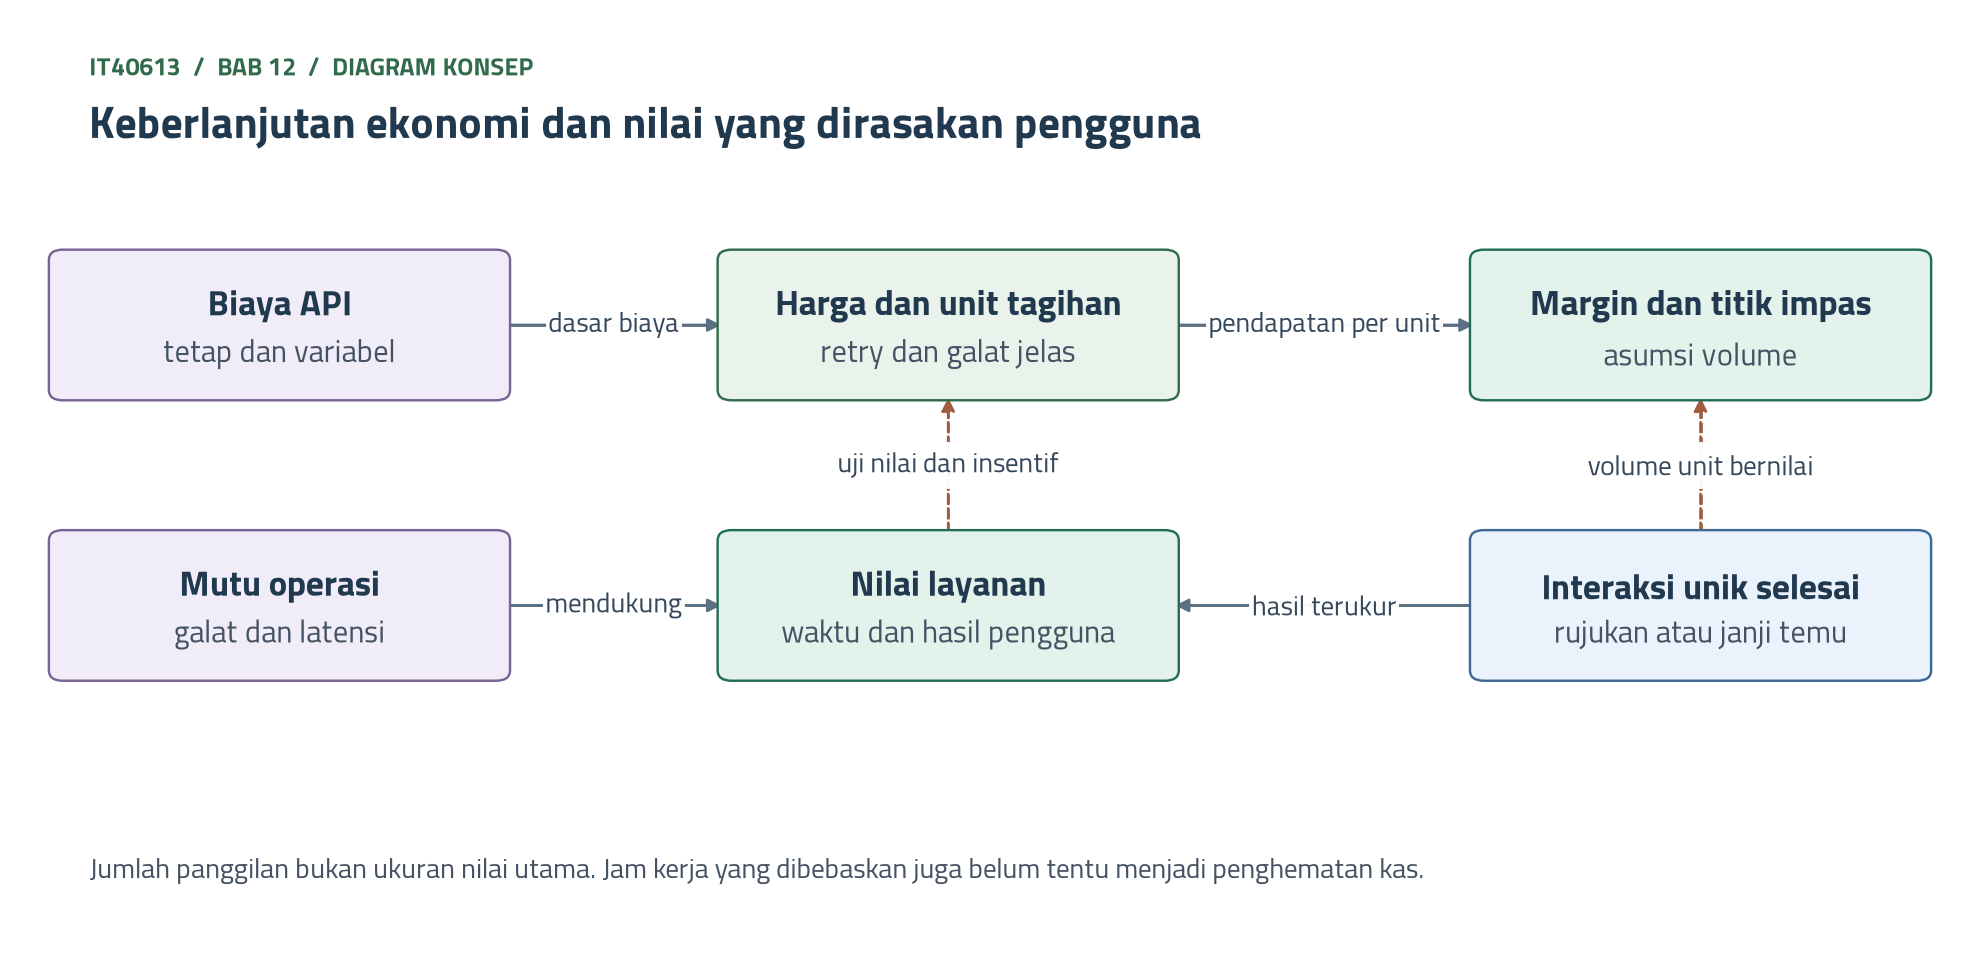
\includegraphics[width=\textwidth]{../figures/ch12-diagram-konsep.png}
  \caption{Keberlanjutan ekonomi dan nilai yang dirasakan pengguna}
  \label{fig:ch12-ilustrasi-bab}
\end{figure}
}{}

Gambar itu memuat dua jalur. Jalur atas adalah jalur ekonomi. Biaya API, baik tetap maupun variabel, menjadi dasar harga dan
unit tagihan. Pendapatan per unit lalu menentukan margin dan titik impas. Jalur bawah adalah jalur layanan. Mutu operasi
mendukung nilai layanan, dan nilai itu terukur lewat interaksi unik yang selesai. Dua panah putus-putus mengikat kedua jalur.
Nilai layanan menguji apakah harga dan insentifnya masuk akal bagi pembayar. Volume unit yang bernilai, bukan volume panggilan,
mengisi hitungan margin.

\section{Nilai API Langsung dan Tidak Langsung}

Bab 4 sudah menyebut bahwa API dapat dijual atau dipakai sendiri. Bagaimana nilai keduanya dibedakan dan dihitung?

Nilai langsung muncul ketika penggunaan API menghasilkan pendapatan yang dapat diatribusikan. Nilai tidak langsung mencakup
perluasan saluran, retensi mitra, atau penghematan proses. Penghematan waktu tidak otomatis menjadi pengurangan kas.
Perhitungan harus menyebut apakah waktu dialihkan, kapasitas bertambah, atau biaya benar-benar dihindari. Laporan Postman 2025
mencatat 65 persen organisasi memperoleh pendapatan dari API, dan 74 persen di antaranya memperoleh minimal 10 persen
pendapatan totalnya dari API \cite{postman2025}. Penerbit laporan itu menjual alat API, sehingga angkanya dibaca sebagai
gambaran pasar, bukan patokan. Benzell dkk. menemukan pertumbuhan tambahan pada perusahaan yang mengadopsi API publik, sedangkan
pemakaian untuk produktivitas internal saja tidak menunjukkan efek signifikan pada ukuran yang sama \cite{benzell2024apis}.
Temuan itu tidak berarti API internal tidak bernilai. Nilainya perlu diukur pada proses yang dilayaninya, bukan pada laporan
keuangan perusahaan secara keseluruhan.

Analoginya jalan penghubung antardesa. Jalan itu bernilai karena truk sayur sampai lebih cepat, walaupun tidak ada loket tol.
Nilainya tidak tercatat di buku kas pengelola jalan, melainkan di buku kas para pedagang.

Dua contoh berangka pada Medikara:
\begin{enumerate}
  \item Misalkan 400 telepon enam menit per bulan dihilangkan. Nilainya 40 jam kapasitas, bukan otomatis penghematan gaji 40
        jam. Pada tarif Rp60.000 per jam, kapasitas itu setara Rp2,4 juta per bulan, atau Rp28,8 juta per tahun. Kas Medikara
        baru berubah bila jam itu menggantikan lembur, tenaga kontrak, atau perekrutan yang dibatalkan.
  \item API pemesanan membantu layanan paket perusahaan terjual. Pendapatan paket perlu dipisahkan dari kontribusi API agar
        tidak dihitung ganda. Bab 4 memisalkan paket 200 karyawan Rp100 juta, dan Medikara menyimpan Rp10 juta. Mencatat
        Rp100 juta sebagai nilai API menggelembungkan angka 10 kali. Rp10 juta pun masih milik seluruh rantai layanan, bukan
        milik API saja.
\end{enumerate}

Dua hal pada nilai tidak langsung sering tertukar, yaitu kapasitas dan kas. Pembagiannya begini. Kas berubah bila ada pembayaran
yang berhenti atau uang yang masuk. Kapasitas berubah bila jam kerja menjadi bebas, sementara gaji tetap dibayar. Tabel
\ref{tab:ch12-jenis-nilai} memisahkan lima klaim nilai beserta bukti yang diminta untuk masing-masing.

\begin{table}[!htb]
  \centering
  \caption{Lima klaim nilai API dan bukti yang diminta. Angka Medikara adalah pemisalan dari bab sebelumnya}
  \label{tab:ch12-jenis-nilai}
  \footnotesize
  \begin{tabularx}{\textwidth}{H{2.15cm}GGH{2.7cm}}
    \hline
    \textbf{Klaim} & \textbf{Arti} & \textbf{Contoh Medikara} & \textbf{Bukti yang diminta} \\ \hline
    Pendapatan baru & Uang masuk karena API dipakai & Verifikasi penjaminan Rp10.000, atau Rp960 juta per tahun pada 96.000 verifikasi (Bab 2). Kontrak belum ada & Tagihan yang direkonsiliasi \\ \hline
    Kas keluar berhenti & Pengeluaran yang benar-benar hilang & Lapisan bersama menurunkan 20 sambungan Rp900 juta menjadi Rp705 juta per tahun (Bab 4), bila sambungan lama dimatikan & Kontrak lama yang berakhir \\ \hline
    Kapasitas dialihkan & Jam kerja bebas, gaji tetap dibayar & Telepon konfirmasi turun dari 10 ke 2 persen: Rp172,8 juta dari Rp216 juta per tahun (Bab 8) & Catatan tugas pengganti \\ \hline
    Risiko berkurang & Peluang kerugian turun & Akses vendor ke 138 tabel yang tidak diperlukan dicabut (Bab 3) & Temuan audit yang ditutup \\ \hline
    Kewajiban dipenuhi & Tanpa API, kewajiban tidak terpenuhi & 10 sambungan ke Badan Penyelenggara Jaminan Sosial (BPJS) Kesehatan dan SATUSEHAT, Rp450 juta per tahun (Bab 4) & Kiriman yang berhasil \\ \hline
  \end{tabularx}
\end{table}

Pembagian ini punya dua konsekuensi. Pertama, laporan manfaat tidak boleh menjumlahkan semua baris tanpa label. Rp172,8 juta dari
telepon yang berkurang terjadi di sisi klinik, sedangkan langganan Rp1,44 miliar adalah imbalan yang dibayar klinik, antara lain
atas penghematan itu. Menjumlahkan keduanya menghitung manfaat yang sama dua kali. Kedua, kapasitas baru menjadi manfaat bila ada
tugas pengganti. Tanpa pemilik yang memutuskan pemakaian jam yang bebas, angka itu hanya ada di kertas.

Ada pula API yang nilainya nol pada semua kolom. Bab 8 mencatat API-06 Identitas dan Akses tanpa manfaat langsung, dengan usaha
1.200 jam, atau Rp72 juta pada tarif Rp60.000 per jam. Namun kandidat API-01 sampai API-04 memakainya sebagai prasyarat. Apakah
API-06 ikut diberi bagian Rp1,44 miliar? Tidak. Manfaatnya dicatat pada tingkat portofolio, supaya satu rupiah tidak diklaim oleh
dua API.

\section{Model Harga API}

Nilai sudah dipetakan. Bentuk harga apa yang menangkap nilai itu tanpa merusaknya?

Model harga meliputi gratis, \textit{freemium}, berjenjang, bayar per pemakaian, dan bagi hasil. Satuan tagihan harus dikenali
pelanggan dan sesuai pemicu biaya. Harga per panggilan mudah diukur, tetapi dapat menghukum pengulangan permintaan (\textit{retry})
akibat galat penyedia. Paket berjenjang memberi kepastian dengan risiko kapasitas menganggur atau lonjakan di atas batas.
API-m-FAMM menuliskan empat model pada area \textit{Commercial}. Pada model langganan, konsumen membayar biaya bulanan tetap dan
boleh memanggil API sampai jumlah tertentu. Pada model berjenjang, tiap jenjang punya layanan dan jatah sendiri, dengan harga
yang naik pada jenjang lebih tinggi. Pada model \textit{freemium}, konsumen memperoleh sebagian layanan, dan layanan penuh
memerlukan langganan berbayar. Pada model meter, yang di sini disebut bayar per pemakaian, konsumen membayar sumber daya yang dipakai, misalnya \textit{bandwidth},
penyimpanan, atau jumlah panggilan \cite{mathijssen2020}. Bagi hasil menambah kemungkinan kelima: penyedia mengambil bagian
dari nilai transaksi.

Analoginya tagihan air dan langganan kelas senam. Tagihan air mengikuti meter, sehingga rumah yang hemat membayar sedikit.
Langganan kelas mengikuti paket kehadiran, sehingga anggota tahu pengeluarannya walaupun tidak selalu datang. Keduanya wajar,
karena kebutuhan pelanggannya berbeda.

Dua contoh berangka pada Medikara:
\begin{enumerate}
  \item API verifikasi dapat dihargai per pemeriksaan yang selesai dan sah, bukan seluruh permintaan termasuk pengulangan
        kesalahan. Bab 2 memisalkan Rp10.000 per verifikasi dan 96.000 verifikasi per tahun, atau Rp960 juta. Misalkan 2 persen
        permintaan diulang karena galat penyedia. Bila ditagih per permintaan, asuransi membayar Rp19,2 juta lebih per tahun
        untuk kesalahan yang bukan miliknya.
  \item Misalkan paket klinik memuat 1.800 janji temu per bulan dengan harga Rp3 juta. Paket itu memberi kepastian bagi klinik dan
        Medikara. Aturan kelebihan kuota dan transaksi gagal harus dinyatakan jelas. Klinik dengan 1.500 janji temu membayar
        Rp2.000 per janji. Klinik dengan 800 janji temu membayar Rp3.750 per janji, dan kelebihan kapasitasnya tidak kembali.
\end{enumerate}

Tabel \ref{tab:ch12-model-harga} merangkum kelima model. Pilihan tidak harus satu. Satu organisasi dapat memakai model berbeda
untuk API dan sisi pasar yang berbeda.

\begin{table}[!htb]
  \centering
  \caption{Lima model harga API dan penerapannya pada Medikara}
  \label{tab:ch12-model-harga}
  \footnotesize
  \begin{tabularx}{\textwidth}{H{1.75cm}GGG}
    \hline
    \textbf{Model} & \textbf{Cocok bila} & \textbf{Risiko} & \textbf{Pada Medikara} \\ \hline
    Gratis & Nilai ditangkap di tempat lain, atau API adalah kewajiban & Biaya berjalan tanpa pemilik anggaran & API internal, sambungan BPJS Kesehatan dan SATUSEHAT \\ \hline
    \textit{Freemium} & Biaya tambahan per pemakai kecil, dan ada alasan alami untuk naik kelas & Pemakai gratis tidak pernah membayar & Tingkat 0 pada Bab 3: jadwal dokter tanpa akun, batas 1.000 panggilan per hari, tanpa data pasien \\ \hline
    Berjenjang & Ukuran pelanggan berbeda, dan pelanggan menginginkan kepastian & Kapasitas menganggur, lonjakan di atas batas & Paket klinik kecil, sedang, dan besar \\ \hline
    Bayar per pemakaian & Volume berubah-ubah, dan unitnya bermakna bagi pelanggan & Tagihan sulit diperkirakan, pendapatan mengikuti volume & Verifikasi penjaminan Rp10.000 per verifikasi \\ \hline
    Bagi hasil & Nilai transaksi terukur, dan penyedia ikut dalam transaksi & Rekonsiliasi rumit, insentif dapat memengaruhi keputusan klinis & Paket perusahaan: Rp10 juta dari Rp100 juta, atau 10 persen \\ \hline
  \end{tabularx}
\end{table}

Harga terbuka memberi gambaran bentuk tagihan di pasar. Tabel \ref{tab:ch12-harga-publik} memuat tiga penyedia yang harganya dapat
dibaca publik. Pasar, mata uang, dan layanannya berbeda dari Medikara, sehingga yang dipelajari adalah bentuknya, bukan besarnya.

\begin{table}[!htb]
  \centering
  \caption{Contoh harga terbuka tiga penyedia API. Diakses 31 Oktober 2026, dan harga dapat berubah}
  \label{tab:ch12-harga-publik}
  \footnotesize
  \begin{tabularx}{\textwidth}{H{2.1cm}H{2.5cm}G}
    \hline
    \textbf{Penyedia} & \textbf{Bentuk} & \textbf{Rincian yang tertulis} \\ \hline
    Stripe \cite{stripe-pricing} & Bagian dari nilai transaksi & 2,9 persen ditambah 30 sen dolar per transaksi kartu domestik yang berhasil pada tarif standar Amerika Serikat. Tanpa biaya pendaftaran dan bulanan. Sengketa 15 dolar per kasus \\ \hline
    Twilio \cite{c12-twilio-sms} & Per pemakaian & 0,0083 dolar per segmen pesan singkat pada nomor panjang Amerika Serikat, ditambah biaya operator. 0,001 dolar untuk pesan yang berakhir berstatus gagal. Potongan volume lewat tim penjualan \\ \hline
    Google Maps Platform \cite{c12-google-maps-pricing} & Gratis sampai batas, lalu per pemakaian atau paket & Panggilan gratis per produk per bulan 10.000, 5.000, atau 1.000 menurut kategori. Potongan otomatis mulai 20 persen di atas 100.000 panggilan pada sebagian besar produk. Paket 100 dolar untuk 50.000 panggilan, 275 dolar untuk 100.000, dan 1.200 dolar untuk 250.000 \\ \hline
  \end{tabularx}
\end{table}

Ketiganya berbeda pada satu hal yang penting bagi Medikara: apa yang terjadi saat transaksi gagal. Stripe menulis tarifnya per
transaksi yang berhasil. Twilio menarik biaya kecil untuk pesan yang berakhir gagal, sekitar 12 persen dari harga dasar per
segmen. Google menulis harganya per panggilan. Pilihan itu menentukan pihak yang menanggung kegagalan.

Mengapa pelanggan sering memilih paket, walaupun per pemakaian bisa lebih murah? Lambrecht dan Skiera menemukan bias menyukai
tarif tetap (\textit{flat-rate bias}) lebih penting dan lebih menetap daripada bias sebaliknya. Bias menyukai tarif tetap tidak
menaikkan perpindahan pelanggan secara berarti, sedangkan bias menyukai bayar per pemakaian menaikkannya
\cite{c12-lambrecht2006}. Sundararajan menunjukkan bahwa menawarkan tarif tetap di samping tarif pemakaian selalu menguntungkan
bila penagihan pemakaian punya biaya transaksi \cite{c12-sundararajan2004}. Kedua artikel tidak ditulis khusus untuk API, sehingga
dipakai sebagai petunjuk, bukan angka baku.

Pertanyaan kemudian muncul: untuk API-01, model mana yang lebih adil? Misalkan 40 klinik terbagi menjadi 10 klinik kecil dengan 20
janji temu per hari, 20 klinik sedang dengan 60 janji temu, dan 10 klinik besar dengan 100 janji temu. Rata-ratanya tetap 60 per
hari, sama dengan Bab 3. Dengan tiga panggilan per pemesanan, klinik besar tepat mencapai kuota 300 panggilan per hari. Tabel
\ref{tab:ch12-tiga-model} dan Gambar \ref{fig:ch12-tagihan} membandingkan tiga model yang disusun supaya pendapatannya sama, yaitu
Rp1,44 miliar per tahun. Seluruh sebaran dan harga di luar Rp3 juta adalah pemisalan latihan, dan dapat diulang dengan
\berkas{sources/chapter12/hitung-monetisasi.py}.

\begin{table}[!htb]
  \centering
  \caption{Tiga model harga API-01 dengan pendapatan yang sama. Harga efektif per janji ditulis dalam kurung}
  \label{tab:ch12-tiga-model}
  \footnotesize
  \begin{tabularx}{\textwidth}{H{1.75cm}H{1.0cm}H{1.5cm}H{1.5cm}GGG}
    \hline
    \textbf{Kelompok} & \textbf{Klinik} & \textbf{Janji per bulan} & \textbf{Panggilan per bulan} & \textbf{Langganan datar} & \textbf{Per janji sah} & \textbf{Berjenjang} \\ \hline
    Kecil & 10 & 500 & 1.500 & Rp3 juta (Rp6.000) & Rp1 juta (Rp2.000) & Rp1,5 juta (Rp3.000) \\ \hline
    Sedang & 20 & 1.500 & 4.500 & Rp3 juta (Rp2.000) & Rp3 juta (Rp2.000) & Rp3 juta (Rp2.000) \\ \hline
    Besar & 10 & 2.500 & 7.500 & Rp3 juta (Rp1.200) & Rp5 juta (Rp2.000) & Rp4,5 juta (Rp1.800) \\ \hline
    \textbf{Per tahun} & \textbf{40} & \textbf{720.000} & \textbf{2.160.000} & \textbf{Rp1,44 miliar} & \textbf{Rp1,44 miliar} & \textbf{Rp1,44 miliar} \\ \hline
  \end{tabularx}
\end{table}

\begin{figure}[!htb]
  \centering
  \begin{tikzpicture}[font=\scriptsize]
  \begin{axis}[
    width=11cm, height=6cm,
    xmin=0, xmax=2600, ymin=0, ymax=6,
    xtick={0,500,750,1500,1800,2500},
    ytick={0,1,1.5,2,3,4,4.5,5,6},
    yticklabels={0,1,{1,5},2,3,4,{4,5},5,6},
    xlabel={Janji temu per bulan per klinik},
    ylabel={Tagihan per bulan (juta rupiah)},
    xticklabel style={/pgf/number format/.cd, 1000 sep={.}},
    tick label style={font=\tiny},
    label style={font=\scriptsize},
    legend style={font=\tiny, at={(0.02,0.98)}, anchor=north west, draw=gray!50},
    legend cell align=left,
    grid=major, grid style={gray!20},
    every axis plot/.append style={thick, mark=none}
  ]
    \addplot[gray!70!black, dashed] coordinates {(0,3) (2500,3)};
    \addlegendentry{langganan datar Rp3 juta}
    \addplot[blue!70!black] coordinates {(0,0) (2500,5)};
    \addlegendentry{per janji sah Rp2.000}
    \addplot[praditagreen, very thick] coordinates {
      (0,1.5) (750,1.5) (750,3) (1800,3) (1800,4.5) (2500,4.5)};
    \addlegendentry{berjenjang: kecil, sedang, besar}
    \node[font=\tiny, anchor=west] at (axis cs:540,0.8) {klinik kecil};
    \node[font=\tiny, anchor=north west] at (axis cs:1500,3) {klinik sedang};
    \node[font=\tiny, anchor=south east] at (axis cs:2500,5) {klinik besar};
    \addplot[only marks, mark=*, mark size=1.3pt, black] coordinates {
      (500,1) (500,1.5) (500,3) (1500,3) (2500,3) (2500,4.5) (2500,5)};
  \end{axis}
\end{tikzpicture}

  \caption{Tagihan klinik pada tiga model. Paket kecil memuat 750 janji, paket sedang 1.800 janji, dan paket besar 2.500 janji}
  \label{fig:ch12-tagihan}
\end{figure}

Totalnya sama, tetapi yang menanggung berbeda. Pada langganan datar, klinik kecil membayar Rp6.000 per janji, atau 5 kali klinik
besar. Pada per janji sah, semua klinik membayar Rp2.000, tetapi tagihan bulanan mengikuti volume dan sulit dianggarkan. Berjenjang
berada di antara keduanya, dengan satu cacat: klinik yang melewati 750 janji langsung naik Rp1,5 juta.

Dua hal pada tagihan sering tertukar, yaitu kuota dan unit tagihan. Pembagiannya begini. Kuota melindungi sistem, sehingga
menghitung setiap permintaan yang datang. Unit tagihan menentukan pembayaran, sehingga hanya menghitung hasil yang bernilai. Bab 10
sudah mengingatkan bahwa kuota di \textit{gateway} bersifat \textit{best-effort}, sehingga penagihan memerlukan catatan pemakaian
yang direkonsiliasi \cite{aws-throttling}. Tabel \ref{tab:ch12-aturan-tagihan} menurunkan aturan itu per jenis jawaban API-01.

\begin{table}[!htb]
  \centering
  \caption{Aturan tagihan API-01 per jenis jawaban. Kuota tetap menghitung seluruh permintaan}
  \label{tab:ch12-aturan-tagihan}
  \footnotesize
  \begin{tabularx}{\textwidth}{GH{1.45cm}G}
    \hline
    \textbf{Jawaban} & \textbf{Ditagih} & \textbf{Alasan} \\ \hline
    201 pertama untuk satu kunci idempotensi & Ya & Satu janji sah terbentuk \\ \hline
    Jawaban ulang dengan kunci idempotensi yang sama & Tidak & Tidak ada janji baru \\ \hline
    409 konflik slot & Tidak & Klinik memperoleh informasi, tetapi janji tidak terbentuk \\ \hline
    401 dan 429 & Tidak & Beban dukungan dan kuota, bukan nilai layanan \\ \hline
    503 dan jawaban 5xx lain & Tidak & Penyedia tidak dibayar atas kegagalannya, dan permintaan masuk hitungan ketersediaan \\ \hline
    200 pada pembacaan jadwal & Tidak & Pembacaan adalah biaya operasi, ditahan dengan kuota dan \textit{cache} \\ \hline
  \end{tabularx}
\end{table}

Aturan ini punya dua konsekuensi. Pertama, penyedia tidak lagi diuntungkan oleh kegagalannya. Misalkan harga Rp667 per panggilan,
yaitu angka setara pada Bab 4, dan 10 persen panggilan diulang karena gangguan penyedia. Panggilan bulanan naik dari 180.000
menjadi 198.000, dan tagihan seluruh klinik naik sekitar Rp12 juta per bulan tanpa satu pun janji baru. Kedua, tagihan per janji
perlu rekonsiliasi. Misalkan satu klinik memerlukan 1 jam per bulan. Untuk 40 klinik, bebannya 480 jam, atau Rp28,8 juta per tahun.
API-m-FAMM juga menuntut prasyarat serupa: model langganan memerlukan sistem pengelolaan langganan dan pengelolaan kuota, sedangkan
model meter memerlukan pemantauan pemakaian \cite{mathijssen2020}.

\section{Harga dalam Pasar Multi-Sisi}

Model harga belum menjawab satu hal. Pada platform dengan beberapa sisi, sisi mana yang seharusnya membayar?

Pada pasar multi-sisi, pembayar tidak harus pihak yang menghasilkan seluruh trafik. Subsidi dapat membantu sisi yang diperlukan untuk
menciptakan interaksi, tetapi memerlukan batas waktu dan ukuran keberhasilan. Harga perlu mempertimbangkan elastisitas, kualitas, dan
efek jaringan negatif. Pertumbuhan yang disubsidi tidak otomatis berkelanjutan. Rochet dan Tirole mengenali pasar dua sisi dari ciri
berikut: struktur harga, bukan hanya tingkat harga, ikut menentukan hasil \cite{c12-rochet2006}. Armstrong menyebut tiga penentu
harga: besarnya pengaruh antarkelompok, apakah biaya ditarik sekaligus atau per transaksi, dan apakah anggota memakai satu atau
beberapa platform \cite{armstrong2006competition}. Evans dan Schmalensee menunjukkan platform harus memperoleh cukup anggota pada kedua sisi
agar berhasil diluncurkan \cite{c12-evans2010}. Bab 2 sudah memakai istilah sisi subsidi dan sisi pembayar dari Eisenmann dkk.
\cite{eisenmann2006strategies}.

Analoginya pameran dagang. Pengelola acara dapat menggratiskan tiket pengunjung karena peserta pameran membayar tempat. Peserta
bersedia membayar selama pengunjung datang. Bila tiket dibuat mahal, pengunjung berkurang, dan peserta pun menolak membayar.

Dua contoh berangka pada Medikara:
\begin{enumerate}
  \item Bab 2 menghitung pembebanan kepada pasien. Rp10.000 per pemesanan membuat 30 persen pasien kembali ke telepon, pemesanan turun
        dari 240.000 menjadi 168.000, dan pendapatan hanya Rp1,68 miliar, kurang Rp720 juta dari biaya Rp2,4 miliar. Bila klinik
        dan asuransi yang membayar, pendapatannya Rp2,4 miliar tanpa menekan pemesanan. Tingkat harganya sama, tetapi strukturnya
        menghasilkan akibat yang berbeda.
  \item Subsidi tanpa verifikasi dapat menarik mitra yang tidak aktif. Masa uji enam bulan pada Bab 2 bernilai Rp18 juta per klinik,
        atau Rp720 juta untuk 40 klinik. Misalkan hanya 28 klinik yang bertahan. Subsidi Rp216 juta tidak kembali, dan subsidi per
        klinik yang bertahan naik dari Rp18 juta menjadi sekitar Rp25,7 juta. Aktivitas sah serta mutu interaksi diukur sesudah subsidi
        berakhir, bukan selama masa gratis.
\end{enumerate}

Gambar \ref{fig:ch12-arus} memperlihatkan arus nilai dan arus uang pada pemisalan Bab 2. Tabel \ref{tab:ch12-sisi-pasar} menambahkan
risiko pada tiap sisi. Vendor sistem klinik ditulis pada tabel, karena 28 klinik mengandalkan 3 vendor menurut Bab 11, walaupun vendor
bukan pihak yang menerima tagihan.

\begin{figure}[!htb]
  \centering
  \begin{tikzpicture}[
  pusat/.style={draw, rounded corners, fill=praditagreen!15, text width=2.7cm,
    minimum height=1.9cm, align=center, font=\scriptsize\bfseries},
  sisi/.style={draw, rounded corners, fill=blue!8, text width=3.1cm,
    minimum height=1.4cm, align=center, font=\scriptsize},
  panah/.style={-{Stealth[length=2mm]}, thick},
  nilai/.style={panah, blue!60!black},
  uang/.style={panah, orange!80!black},
  nol/.style={panah, gray!60!black, dashed}
]
  \node[pusat] (p) at (0,0) {Medikara+ dan API-01\\
    {\tiny\mdseries Biaya Rp2,4 miliar per tahun, pemisalan Bab 2}};
  \node[sisi] (pasien) at (-4.2,1.2) {\textbf{Pasien}\\
    {\tiny\mdseries Menerima janji tanpa antre telepon. Rp0 untuk pemesanan}};
  \node[sisi] (asuransi) at (-4.2,-1.2) {\textbf{Asuransi swasta}\\
    {\tiny\mdseries Menerima verifikasi otomatis. Rp10.000 per verifikasi, Rp960 juta}};
  \node[sisi] (klinik) at (4.2,1.2) {\textbf{Klinik mitra}\\
    {\tiny\mdseries Menerima pasien dan telepon lebih sedikit. Rp3 juta per bulan, Rp1,44 miliar}};
  \node[sisi] (perusahaan) at (4.2,-1.2) {\textbf{Perusahaan klien}\\
    {\tiny\mdseries Menerima layanan karyawan. Paket per karyawan pada Tahap 3}};
  \draw[nilai] ([yshift=0.55cm]p.west) -- ([yshift=0.12cm]pasien.east);
  \draw[nol] ([yshift=-0.12cm]pasien.east) -- ([yshift=0.25cm]p.west);
  \draw[nilai] ([yshift=-0.25cm]p.west) -- ([yshift=0.12cm]asuransi.east);
  \draw[uang] ([yshift=-0.12cm]asuransi.east) -- ([yshift=-0.55cm]p.west);
  \draw[nilai] ([yshift=0.55cm]p.east) -- ([yshift=0.12cm]klinik.west);
  \draw[uang] ([yshift=-0.12cm]klinik.west) -- ([yshift=0.25cm]p.east);
  \draw[nilai] ([yshift=-0.25cm]p.east) -- ([yshift=0.12cm]perusahaan.west);
  \draw[uang] ([yshift=-0.12cm]perusahaan.west) -- ([yshift=-0.55cm]p.east);
  \draw[nilai] (-4.3,-2.45) -- (-3.5,-2.45)
    node[right, font=\tiny, text=black] {nilai yang diterima};
  \draw[uang] (-0.9,-2.45) -- (-0.1,-2.45)
    node[right, font=\tiny, text=black] {uang yang dibayar};
  \draw[nol] (2.4,-2.45) -- (3.2,-2.45)
    node[right, font=\tiny, text=black] {tanpa bayaran};
\end{tikzpicture}

  \caption{Arus nilai dan arus uang pada empat sisi Medikara+, dengan pemisalan Bab 2 dan Bab 4}
  \label{fig:ch12-arus}
\end{figure}

\begin{table}[!htb]
  \centering
  \caption{Siapa menerima nilai dan siapa membayar pada Medikara+. Angka adalah pemisalan bab sebelumnya}
  \label{tab:ch12-sisi-pasar}
  \footnotesize
  \begin{tabularx}{\textwidth}{H{1.8cm}GH{2.7cm}H{2.05cm}G}
    \hline
    \textbf{Sisi} & \textbf{Nilai yang diterima} & \textbf{Yang dibayar} & \textbf{Per tahun} & \textbf{Risiko bila harga naik} \\ \hline
    Pasien & Janji tanpa antre telepon & Rp0 untuk pemesanan, tarif konsultasi tetap & Rp0 & 30 persen kembali ke telepon pada Rp10.000 \\ \hline
    Klinik mitra & Pasien lewat aplikasi, telepon berkurang & Rp3 juta per bulan sesudah masa uji & Rp1,44 miliar & Klinik berhenti: Rp36 juta per klinik \\ \hline
    Asuransi swasta & Verifikasi otomatis & Rp10.000 per verifikasi & Rp960 juta & Kontrak dengan 9 asuransi belum ada \\ \hline
    Perusahaan klien & Layanan karyawan & Paket per karyawan mulai Tahap 3 & Belum dihitung & Marjin Rp10 juta per 200 karyawan menipis \\ \hline
    Vendor sistem klinik & Satu integrasi untuk rata-rata 9 klinik & Rp0 & Rp0 & Bila ditagih, beban pindah ke 28 klinik \\ \hline
  \end{tabularx}
\end{table}

Dua hal pada subsidi sering tertukar, yaitu \textit{freemium} dan masa uji. Pembagiannya begini. \textit{Freemium} memberi sebagian
kemampuan tanpa batas waktu. Tingkat 0 pada Bab 3 termasuk bentuk ini. Masa uji memberi kemampuan penuh selama waktu terbatas.
Keduanya punya biaya yang berbeda. Tingkat 0 hanya membebani jadwal yang tidak memuat data pasien, sedangkan masa uji menunda
pendapatan Rp720 juta. Bab 2 juga menuntut tiap subsidi ditulis bersama tujuan dan syarat berhentinya.

Berapa harga yang masuk akal bagi klinik? Itulah uji nilai dan insentif pada Gambar \ref{fig:ch12-ilustrasi-bab}. Tabel
\ref{tab:ch12-uji-nilai} menghitung nilai telepon yang berkurang dari 10 ke 2 persen, seperti ukuran janji nilai API-01 pada Bab 8, dengan
3 menit per telepon dan tarif Rp60.000 per jam. Misalkan satu kunjungan tambahan memberi marjin Rp40.000 bagi klinik.

\begin{table}[!htb]
  \centering
  \caption{Uji nilai bagi klinik: kunjungan tambahan yang diperlukan agar tagihan tertutup. Marjin Rp40.000 adalah pemisalan latihan}
  \label{tab:ch12-uji-nilai}
  \footnotesize
  \begin{tabularx}{\textwidth}{GH{1.45cm}H{1.45cm}H{1.4cm}H{1.45cm}H{1.45cm}H{1.25cm}}
    \hline
    \textbf{Kelompok dan model} & \textbf{Telepon berkurang} & \textbf{Nilai telepon} & \textbf{Tagihan} & \textbf{Sisa yang ditutup} & \textbf{Kunjungan tambahan} & \textbf{Terhadap janji} \\ \hline
    Kecil, langganan datar & 40 & Rp120.000 & Rp3 juta & Rp2,88 juta & 72 & 14,4 persen \\ \hline
    Kecil, berjenjang & 40 & Rp120.000 & Rp1,5 juta & Rp1,38 juta & 35 & 7,0 persen \\ \hline
    Sedang, kedua model & 120 & Rp360.000 & Rp3 juta & Rp2,64 juta & 66 & 4,4 persen \\ \hline
    Besar, langganan datar & 200 & Rp600.000 & Rp3 juta & Rp2,4 juta & 60 & 2,4 persen \\ \hline
    Besar, berjenjang & 200 & Rp600.000 & Rp4,5 juta & Rp3,9 juta & 98 & 3,9 persen \\ \hline
  \end{tabularx}
\end{table}

\begin{kasus}[title={Kasus Medikara Health: Mengapa Klinik Mau Membayar Rp3 Juta?}]
Misalkan Manajer Keuangan, pemilik kemitraan, dan Manajer Layanan Rawat Jalan membaca Tabel \ref{tab:ch12-uji-nilai}. Seluruh rincian ini
adalah data latihan. Pemilik kemitraan semula yakin penghematan telepon sudah cukup untuk menjual langganan. Angkanya tidak mendukung.
Bagi klinik sedang, telepon yang berkurang bernilai Rp360.000 per bulan, atau 12 persen dari tagihan. Sisanya hanya masuk akal bila
Medikara+ benar-benar mengirim pasien, sesuai peringatan Bab 2.

Tim membaca dua hal. Pertama, beban pada langganan datar tidak merata. Klinik kecil memerlukan tambahan 14,4 persen, sedangkan klinik
besar hanya 2,4 persen. Klinik kecil paling mungkin berhenti. Kedua, berjenjang mempersempit rentang itu menjadi 3,9 sampai 7,0
persen dengan total pendapatan yang sama.

Rapat menghasilkan empat keputusan.
\begin{enumerate}
  \item Pasien tetap Rp0 untuk pemesanan. Vendor tidak ditagih.
  \item Klinik dikenai paket berjenjang dengan unit janji sah. Paket sedang tetap Rp3 juta, sehingga angka Bab 2 berlaku sebagai harga
        rata-rata. Keputusan ini bersyarat pada sebaran klinik nyata sesudah 6 bulan.
  \item Masa uji tetap enam bulan. Klinik yang belum punya satu 201 produksi dalam 30 hari menerima pendampingan, bukan perpanjangan.
  \item Bagi hasil atas rujukan ditolak untuk saat ini. Insentif itu dapat memengaruhi keputusan klinis, dan tim hukum perlu memeriksa
        aturan yang berlaku sebelum pilihan itu dibuka lagi.
\end{enumerate}

Pilihan ini punya harga. Pendapatan menjadi peka terhadap sebaran klinik. Bila klinik kecil ternyata 20 dan klinik besar 0, sementara
klinik sedang tetap 20, pendapatan bulanan turun dari Rp120 juta menjadi Rp90 juta, atau Rp1,08 miliar per tahun. Bukti yang dapat mengubah
keputusan adalah sebaran nyata, kunjungan tambahan yang teramati, serta jawaban klinik pada wawancara kesediaan membayar.
\end{kasus}

\section{Biaya dan Titik Impas API}

Harga dan pembayar sudah dipilih. Apakah hasilnya menutup biaya, dan biaya yang mana?

Titik impas menghubungkan biaya tetap, biaya variabel, harga, dan volume yang dapat ditagih. Rumus sederhana volume impas adalah biaya
tetap dibagi selisih harga dan biaya variabel per unit. Selisih itu disebut margin per unit. Rumus hanya berlaku bila margin positif
dan asumsi kapasitas masih masuk akal. Biaya keamanan, dukungan, serta pengiriman data tidak boleh diabaikan.
\begin{equation*}
  \text{Volume impas} = \frac{\text{Biaya tetap}}{\text{Harga per unit} - \text{Biaya variabel per unit}}
\end{equation*}

Analoginya warung makan. Warung menghitung berapa porsi yang perlu terjual untuk menutup sewa setelah biaya bahan dipenuhi. Bila
harga satu porsi sama dengan biaya bahannya, warung tetap rugi sebanyak sewa, seramai apa pun pembelinya.

Dua contoh berangka:
\begin{enumerate}
  \item Misalkan biaya tetap Rp20 juta per bulan, harga Rp500 per unit, dan biaya variabel Rp100. Margin Rp400. Titik impas 50.000
        unit per bulan.
  \item Jika harga turun menjadi Rp100, margin menjadi nol. Tidak ada volume terbatas yang menutup biaya tetap pada model tersebut.
\end{enumerate}

Bagaimana angka itu pada API-01? Tabel \ref{tab:ch12-biaya} menyusun biayanya. Pagu Rp300 juta pada Bab 4 dan Bab 10 bukan seluruhnya
biaya tetap. Bab 10 memisalkan Rp60 juta dari langganan \textit{gateway} bergantung pada trafik, dan Bab 11 memasukkan tiket Rp14,4
juta pada pilihan portal P2. Keduanya naik bila klinik bertambah. Sisanya, Rp225,6 juta, diperlakukan sebagai bagian tetap. Rata-rata
alternatif A Rp269,6 juta per tahun, ditambah rata-rata P2 Rp29,2 juta, memang masih masuk dalam pagu itu. Seluruh lapisan dibebankan ke
API-01 sebagai asumsi hati-hati, karena lapisan itu juga akan dipakai API lain. Kredit \textit{Service Level Agreement} (SLA) dicatat Bab
11 sebagai pengurang pendapatan, dan hitungan ini memperlakukannya seperti biaya variabel agar rumusnya tetap satu.

\begin{table}[!htb]
  \centering
  \caption{Biaya tahunan API-01 pada 40 klinik, dalam juta rupiah. Tersedia di \berkas{sources/chapter12/kalkulator-biaya-api.csv}}
  \label{tab:ch12-biaya}
  \footnotesize
  \begin{tabularx}{\textwidth}{H{4.6cm}H{1.3cm}H{1.3cm}G}
    \hline
    \textbf{Komponen} & \textbf{Jenis} & \textbf{Nilai} & \textbf{Asal angka} \\ \hline
    Lapisan bersama, bagian tetap & Tetap & 225,6 & Pagu Rp300 juta dikurangi trafik dan tiket \\ \hline
    Pemilik produk, dukungan, dan perubahan & Tetap & 180 & Misalkan setara API klaim pada Bab 4 \\ \hline
    \textbf{Jumlah biaya tetap} & & \textbf{405,6} & \\ \hline
    Trafik & Variabel & 60 & Bab 10 \\ \hline
    Tiket dukungan & Variabel & 14,4 & Bab 11: 1 tiket per klinik per bulan, 30 menit \\ \hline
    Rekonsiliasi tagihan & Variabel & 28,8 & Misalkan 1 jam per klinik per bulan \\ \hline
    Kredit SLA & Variabel & 12 & Bab 11: 1 bulan meleset per tahun \\ \hline
    \textbf{Jumlah biaya variabel} & & \textbf{115,2} & Rp2,88 juta per klinik \\ \hline
    \textbf{Total pada 40 klinik} & & \textbf{520,8} & \\ \hline
  \end{tabularx}
\end{table}

Harga rata-rata Rp3 juta per bulan berarti Rp36 juta per klinik per tahun. Margin per klinik Rp33,12 juta. Titik impasnya Rp405,6 juta
dibagi Rp33,12 juta, atau 12,25 klinik, sehingga dibulatkan menjadi 13 klinik. Gambar \ref{fig:ch12-impas} memperlihatkan titik itu.
Pada 12 klinik, lapisan API rugi Rp8,16 juta. Pada 13 klinik, untung Rp24,96 juta. Pada 40 klinik, marginnya Rp919,2 juta.

\begin{figure}[!htb]
  \centering
  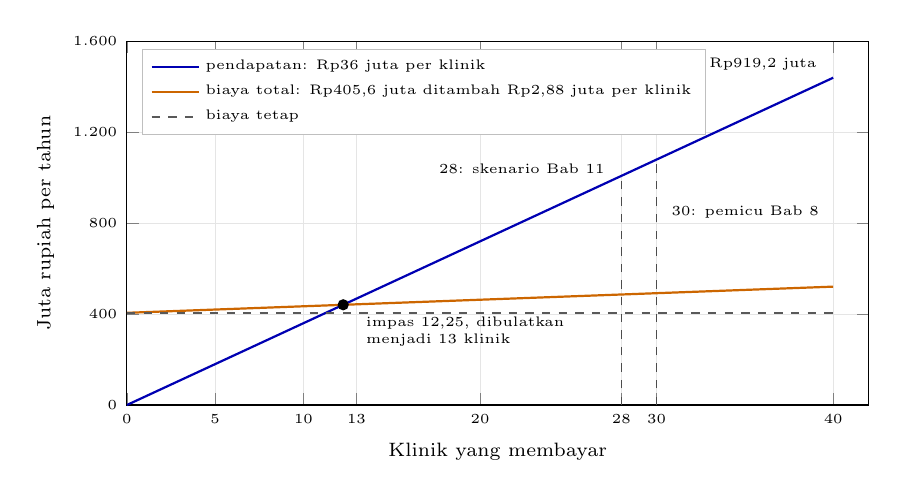
\begin{tikzpicture}[font=\scriptsize]
  \begin{axis}[
    width=11cm, height=6.2cm,
    xmin=0, xmax=42, ymin=0, ymax=1600,
    xtick={0,5,10,13,20,28,30,40},
    ytick={0,400,800,1200,1600},
    xlabel={Klinik yang membayar},
    ylabel={Juta rupiah per tahun},
    yticklabel style={/pgf/number format/.cd, 1000 sep={.}},
    scaled y ticks=false,
    tick label style={font=\tiny},
    label style={font=\scriptsize},
    legend style={font=\tiny, at={(0.02,0.98)}, anchor=north west, draw=gray!50},
    legend cell align=left,
    grid=major, grid style={gray!20},
    every axis plot/.append style={thick, mark=none}
  ]
    \addplot[blue!70!black] coordinates {(0,0) (40,1440)};
    \addlegendentry{pendapatan: Rp36 juta per klinik}
    \addplot[orange!80!black] coordinates {(0,405.6) (40,520.8)};
    \addlegendentry{biaya total: Rp405,6 juta ditambah Rp2,88 juta per klinik}
    \addplot[gray!70!black, dashed] coordinates {(0,405.6) (40,405.6)};
    \addlegendentry{biaya tetap}
    \addplot[only marks, mark=*, mark size=1.6pt, black] coordinates {(12.25,441)};
    \node[font=\tiny, anchor=north west, align=left] at (axis cs:13,430)
      {impas 12,25, dibulatkan\\ menjadi 13 klinik};
    \draw[gray!60!black, dashed] (axis cs:28,0) -- (axis cs:28,1008);
    \draw[gray!60!black, dashed] (axis cs:30,0) -- (axis cs:30,1080);
    \node[font=\tiny, anchor=east, align=right] at (axis cs:27.6,1040)
      {28: skenario Bab 11};
    \node[font=\tiny, anchor=west, align=left] at (axis cs:30.3,850)
      {30: pemicu Bab 8};
    \node[font=\tiny, anchor=east] at (axis cs:39.6,1500)
      {40: margin Rp919,2 juta};
  \end{axis}
\end{tikzpicture}

  \caption{Titik impas lapisan API-01 menurut jumlah klinik yang membayar. Seluruh angka adalah pemisalan latihan}
  \label{fig:ch12-impas}
\end{figure}

Seberapa kuat angka 13 itu? Tabel \ref{tab:ch12-kepekaan} mengubah satu asumsi setiap kali. Harga jauh lebih menentukan daripada trafik.
Pada Rp1 juta per bulan, titik impasnya 45 klinik, atau lebih banyak daripada seluruh klinik mitra. Pada Rp240.000 per bulan, margin
menjadi nol, sama seperti contoh warung tadi. Trafik dua kali lipat tidak mengubah hasil pembulatan. Pada Bab 10, kenaikan trafik itu
mengancam pagu. Pada bab ini, kenaikan yang sama tidak mengancam titik impas, karena pendapatan klinik jauh lebih besar daripada biaya
trafik per klinik. Kedua kesimpulan benar, dan menjawab pertanyaan yang berbeda.

\begin{table}[!htb]
  \centering
  \caption{Kepekaan titik impas API-01. Satu asumsi diubah pada tiap baris}
  \label{tab:ch12-kepekaan}
  \footnotesize
  \begin{tabularx}{\textwidth}{GH{2.45cm}H{2.45cm}H{1.85cm}}
    \hline
    \textbf{Skenario} & \textbf{Biaya tetap} & \textbf{Margin per klinik} & \textbf{Titik impas} \\ \hline
    Dasar: Rp3 juta per bulan & Rp405,6 juta & Rp33,12 juta & 13 klinik \\ \hline
    Harga Rp2 juta per bulan & Rp405,6 juta & Rp21,12 juta & 20 klinik \\ \hline
    Harga Rp1 juta per bulan & Rp405,6 juta & Rp9,12 juta & 45 klinik \\ \hline
    Harga Rp240.000 per bulan & Rp405,6 juta & Rp0 & Tidak ada \\ \hline
    Trafik dua kali lipat & Rp405,6 juta & Rp31,62 juta & 13 klinik \\ \hline
    Tim produk dua kali lipat & Rp585,6 juta & Rp33,12 juta & 18 klinik \\ \hline
    Seluruh pagu dianggap tetap & Rp480 juta & Rp34,98 juta & 14 klinik \\ \hline
  \end{tabularx}
\end{table}

Bagaimana bila harganya per janji sah? Unit impasnya berpindah dari klinik ke janji temu. Biaya Rp520,8 juta dibagi Rp2.000 menghasilkan
260.400 janji per tahun, atau 21.700 per bulan. Di sini muncul masalah yang menarik, karena bab sebelumnya memakai tiga volume dengan
lingkup berbeda. Tabel \ref{tab:ch12-volume} menyandingkannya. Biaya trafik dibiarkan Rp60 juta pada ketiga baris, sehingga hitungan ini
sedikit melebihkan biaya pada volume rendah.

\begin{table}[!htb]
  \centering
  \caption{Pendapatan per janji sah Rp2.000 pada angka dasar 28.000 janji per bulan dan dua skenario dari bab sebelumnya. Titik impas 21.700 janji per bulan}
  \label{tab:ch12-volume}
  \footnotesize
  \begin{tabularx}{\textwidth}{H{1.5cm}GH{2.1cm}H{2.1cm}H{2.1cm}}
    \hline
    \textbf{Asal} & \textbf{Lingkup angka} & \textbf{Janji per bulan} & \textbf{Pendapatan per tahun} & \textbf{Sisa terhadap Rp520,8 juta} \\ \hline
    Bab 8 & Skenario atas: seluruh 60 kunjungan per hari pada 40 klinik memesan lewat API & 60.000 & Rp1,44 miliar & Rp919,2 juta \\ \hline
    Bab 1 dan 5 & Angka dasar: janji temu pada Medikara+ & 28.000 & Rp672 juta & Rp151,2 juta \\ \hline
    Bab 2 & Skenario harga: 240.000 pemesanan per tahun pada 40 klinik mitra & 20.000 & Rp480 juta & Kurang Rp40,8 juta \\ \hline
  \end{tabularx}
\end{table}

Tabel itu memperjelas pihak yang menanggung risiko volume. Per janji sah memindahkan risiko ke Medikara. Langganan datar memindahkannya
ke klinik. Pada 20.000 janji per bulan, rata-rata satu klinik hanya punya 500 janji, sehingga langganan Rp3 juta setara Rp6.000 per
janji. Selama volume belum diketahui, angka mana pun yang dipakai harus diberi tanda asalnya.

\begin{kasus}[title={Kasus Medikara Health: Titik Impas API-01 Bukan Titik Impas Platform}]
Misalkan pada rapat anggaran seorang manajer berkata, ``API-01 impas pada 13 klinik, jadi kehilangan 12 klinik tidak berbahaya.''
Seluruh rincian ini adalah data latihan. Apakah kesimpulannya benar?

Dua titik impas sering tertukar di sini. Titik impas lapisan API menutup Rp520,8 juta pada 40 klinik. Titik impas platform menutup biaya
Medikara+ bagi mitra, yaitu Rp2,4 miliar pada pemisalan Bab 2, yang termasuk biaya lapisan. Pada Bab 2, Rp1,44 miliar langganan ditambah
Rp960 juta verifikasi tepat menutup angka itu, tanpa sisa. Pada 28 klinik, langganan hanya Rp1,008 miliar, dan platform kurang Rp432
juta, walaupun lapisan API mencatat margin Rp521,76 juta. Pada 30 klinik, yaitu pemicu pensiun API-01 pada Bab 8, kurangnya Rp360
juta. Tanpa kontrak verifikasi, kurangnya Rp960 juta. Pada tahun pertama, masa uji enam bulan juga menahan langganan menjadi Rp720 juta.

Kekeliruan manajer itu berasal dari atribusi. Langganan Rp3 juta bukan harga API saja. Klinik membayar pasien yang datang lewat
aplikasi dan layanan di sekitarnya. Margin lapisan API tidak boleh dibaca sebagai laba API.

Rapat menghasilkan tiga keputusan.
\begin{enumerate}
  \item Laporan bulanan memisahkan margin lapisan API dari margin platform.
  \item Angka 13 klinik dipakai sebagai batas bawah keberlanjutan lapisan. Pemicu 30 klinik pada Bab 8 tetap berlaku, karena pemicu itu
        menjaga ekosistem, bukan hanya biaya lapisan.
  \item Tagihan murni per janji ditolak pada tahun pertama. Pada volume Bab 2, pendapatannya kurang Rp40,8 juta dari biaya lapisan,
        dan volume nyata belum ada.
\end{enumerate}

Bukti yang dapat mengubah keputusan adalah volume janji pada 3 bulan pertama sesudah masa uji, harga nyata \textit{gateway}, dan kontrak
pertama dengan asuransi. Rincian kelayakan investasi dibahas pada \textit{business case} di IT40513.
\end{kasus}

\section{Metrik Platform dan Metrik API}

Titik impas bergantung pada klinik yang bertahan. Angka apa yang memberi tahu lebih awal bahwa klinik akan berhenti?

Metrik platform menilai mutu interaksi, seperti likuiditas, tingkat kecocokan permintaan dan penyedia, aktivasi mitra, retensi, serta layanan
selesai. Metrik API menilai adopsi, volume panggilan, dan mutu operasi, yaitu tingkat galat dan latensi. Keduanya dihubungkan melalui identitas transaksi yang aman.
Ukuran teknis yang baik belum membuktikan pasien menerima layanan yang tepat. Parker dkk. menekankan likuiditas, mutu kecocokan, dan kepercayaan
pada tahap awal platform \cite{parker2016platform}. API-m-FAMM mengukur keterlibatan konsumen antara lain dari pengguna unik, pengembang terdaftar,
pengembang aktif, dan aplikasi aktif \cite{mathijssen2020}. Buku \textit{Site Reliability Engineering} menyebut empat sinyal utama, yaitu
latensi, trafik, galat, dan saturasi \cite{c12-sre-monitoring}. Rodden dkk. menyusun proses memetakan tujuan produk ke metrik yang berpusat pada
pengguna \cite{c12-rodden2010}.

Analoginya kasir toko. Kecepatan kasir perlu dibaca bersama jumlah pelanggan yang menerima barang sesuai pesanan. Kasir yang cepat tetapi sering
salah memasukkan barang membuat antrean baru di loket pengembalian.

Dua contoh berangka pada Medikara:
\begin{enumerate}
  \item Satu juta panggilan dapat berasal dari \textit{polling} atau pengulangan galat. Volume harus dibaca bersama jumlah transaksi unik yang selesai.
        Misalkan klinik menanyakan jadwal tiap 6 menit selama 12 jam layanan, seperti hitungan \textit{polling} pada Bab 5. Ada tambahan 120 panggilan,
        sehingga panggilan per klinik naik dari 180 menjadi 300 per hari, atau naik 67 persen, dan masih di dalam kuota. Untuk 40 klinik, panggilan
        bulanan naik dari 180.000 menjadi 300.000 tanpa satu pun janji baru.
  \item Aktivasi mitra diukur dari mitra yang menyelesaikan tugas sah, bukan akun yang pernah dibuat. Bab 11 menunjukkan 40 klinik selalu terlihat aktif
        bila aktif berarti pernah menerima kredensial. Dengan definisi minimal satu 201 produksi dalam 30 hari, angkanya dapat turun menjadi 28. Selisih 12 klinik itu
        setara Rp432 juta per tahun.
\end{enumerate}

Tabel \ref{tab:ch12-metrik} menyusun delapan metrik. Empat baris atas menjawab apakah interaksinya bernilai. Empat baris bawah menjawab apakah salurannya
sehat. Sebagian datanya berasal dari Sistem Informasi Manajemen Rumah Sakit (SIMRS). Definisi aktivasi mengikuti Bab 11. Angka lain adalah pemisalan latihan.

\begin{table}[!htb]
  \centering
  \caption{Delapan metrik pada API-01 beserta sumber data dan cara angkanya menyesatkan. Angka adalah pemisalan latihan}
  \label{tab:ch12-metrik}
  \footnotesize
  \begin{tabularx}{\textwidth}{H{1.75cm}GH{1.65cm}H{1.45cm}G}
    \hline
    \textbf{Metrik} & \textbf{Definisi} & \textbf{Sumber data} & \textbf{Contoh} & \textbf{Menyesatkan bila} \\ \hline
    Likuiditas & Pencarian jadwal yang menemukan minimal satu slot dalam 7 hari & \textit{Gateway}, SIMRS & 85 persen & Jadwal kosong saat pembaruan ikut dihitung \\ \hline
    Tingkat kecocokan & Pemesanan yang memperoleh slot tanpa konflik dalam sasaran waktu & \textit{Gateway}, SIMRS & 90 persen & Sasaran waktu dilonggarkan \\ \hline
    Aktivasi mitra & Klinik dengan minimal satu 201 produksi dalam 30 hari & \textit{Gateway} & 28 dari 40 & Klinik memesan uji di produksi \\ \hline
    Retensi & Klinik aktif 6 bulan lalu yang masih aktif sekarang & \textit{Gateway}, keuangan & 26 dari 28 & Masa gratis dihitung sebagai bertahan \\ \hline
    Adopsi & Klinik yang memegang kredensial produksi & Portal & 34 dari 40 & Kredensial dibaca sebagai pemakaian \\ \hline
    Volume panggilan & Seluruh permintaan per bulan & \textit{Gateway} & 84.000 & \textit{Polling} dan pengulangan terbaca sebagai pertumbuhan \\ \hline
    Tingkat galat & Permintaan pemesanan berkode 5xx dibagi seluruh permintaan pemesanan & \textit{Gateway} & 0,6 persen & Pemeliharaan dan 4xx dicampur tanpa aturan \\ \hline
    Latensi & Persentil ke-95 pemesanan berhasil, dipisah dari yang gagal & \textit{Gateway} & 1.890 ms pada \textit{log}contoh & Dibaca sebagai rata-rata \\ \hline
  \end{tabularx}
\end{table}

Dua hal pada bahasan ini sering tertukar, yaitu metrik API yang sehat dan platform yang sehat. Pembagiannya begini. API dapat memenuhi \textit{Service
Level Objective} (SLO) 99,4 persen, sementara telepon konfirmasi tetap 10 persen. Bab 8 menyebut keadaan itu sebagai hipotesis kanvas yang salah,
walaupun API-nya bekerja sempurna. Sebaliknya, klinik dapat terus memesan sambil menahan galat 5xx yang lambat. SRE mengingatkan bahwa galat yang lambat
lebih buruk daripada galat yang cepat, dan menyarankan latensi berhasil dipisahkan dari latensi gagal \cite{c12-sre-monitoring}.

Bagaimana semua angka itu terlihat pada data? Tabel \ref{tab:ch12-log} membaca \textit{log}\textit{gateway} sintetis dari klinik uji U1 sampai U5. Bila klinik
diurutkan menurut panggilan, U3 tampak paling unggul. Bila diurutkan menurut transaksi unik, U1 yang paling unggul, sedangkan U3 berada di urutan ketiga.
U5 mengirim 5 panggilan, seluruhnya 401, dan tidak menghasilkan janji apa pun. Di data gabungan, tingkat galat 5xx hanya 4,8 persen dan seluruh klinik
terlihat memanggil API, tetapi satu dari lima klinik belum aktif.

\begin{table}[!htb]
  \centering
  \caption{Panggilan dan transaksi unik per klinik uji dari \berkas{sources/chapter12/contoh-log-gateway.csv}. Data sintetis}
  \label{tab:ch12-log}
  \footnotesize
  \begin{tabularx}{\textwidth}{H{1.3cm}H{1.6cm}H{1.6cm}H{1.9cm}G}
    \hline
    \textbf{Klinik} & \textbf{Panggilan} & \textbf{Transaksi unik} & \textbf{Panggilan per transaksi} & \textbf{Yang terlihat pada \textit{log}} \\ \hline
    U1 & 15 & 5 & 3,00 & Pola normal: tiga panggilan per pemesanan \\ \hline
    U2 & 13 & 4 & 3,25 & Satu 503, lalu berhasil dengan kunci yang sama \\ \hline
    U3 & 19 & 3 & 6,33 & Menanyakan jadwal tiap 5 menit \\ \hline
    U4 & 10 & 2 & 5,00 & Dua 503 berturut-turut, satu 409 \\ \hline
    U5 & 5 & 0 & Tidak terhitung & Seluruh jawaban 401, masalah token \\ \hline
    \textbf{Jumlah} & \textbf{62} & \textbf{14} & \textbf{4,43} & Tagihan Rp41.354 per panggilan, Rp28.000 per janji \\ \hline
  \end{tabularx}
\end{table}

Baris terakhir menghubungkan metrik dengan harga. Untuk nilai yang sama, yaitu 14 janji, tagihan per panggilan lebih besar 48 persen daripada tagihan
per janji. Selisih itu berasal dari \textit{polling}, pengulangan, dan permintaan yang ditolak. Pada \textit{log}yang sama, latensi pemesanan berhasil memiliki
median 259 ms dan persentil ke-95 sebesar 1.890 ms, sedangkan rata-rata seluruh pemesanan 722 ms. Angka rata-rata itu tidak menggambarkan pengalaman
klinik mana pun, karena mencampur jawaban cepat, jawaban lambat, dan penolakan. SRE menyarankan histogram latensi, bukan rata-rata
\cite{c12-sre-monitoring}. Sampel 14 pemesanan terlalu kecil untuk persentil ke-95 yang stabil, sehingga angka itu hanya contoh cara membaca.

\begin{pendalaman}[title={Pendalaman Teknis (opsional): Bahan Dashboard Metrik API dari Log Gateway}]
Pendalaman ini menyusun bahan \textit{dashboard} dari \textit{log}\textit{gateway}. Skrip memisahkan panggilan dari transaksi unik, lalu memisahkan latensi berhasil
dari latensi gagal. Listing \ref{lst:ch12-metrik} memuat dua fungsi intinya. \textit{Log} memakai kunci semu pada kolom \texttt{id\_transaksi} dan tidak memuat data pasien.

\textbf{Peringatan.} Pakai hanya \textit{log} sintetis atau \textit{log} berizin yang sudah dianonimkan. \textit{Log} nyata tidak boleh memuat identitas pasien.

\begin{lstlisting}[style=ch12python, caption={Menghitung transaksi unik dan persentil dari \textit{log}, tersedia di \berkas{sources/chapter12/hitung-metrik-gateway.py}}, label={lst:ch12-metrik}]
def persentil(nilai, persen):
  """Peringkat terdekat, karena sampel kecil tidak perlu interpolasi."""
  urutan = sorted(nilai)
  peringkat = math.ceil(persen / 100 * len(urutan))
  return urutan[peringkat - 1]


def transaksi_unik(baris_log):
  """Menghitung janji sah per id, agar pengulangan tidak terhitung dua."""
  return {
    baris["id_transaksi"]
    for baris in baris_log
    if baris["operasi"] == OPERASI_PEMESANAN
    and int(baris["status"]) == STATUS_TERBENTUK
  }
\end{lstlisting}

Susun \textit{dashboard} menjadi lima panel, dari yang paling dekat dengan nilai: interaksi unik selesai per minggu, klinik aktif dan klinik tanpa transaksi
30 hari, panggilan per transaksi per klinik, galat 5xx terhadap SLO 99,4 persen, dan latensi persentil ke-50 serta ke-95 yang memisahkan jawaban berhasil dari
jawaban gagal. Urutan panel menentukan rapat. Panel pertama yang dibaca adalah pertanyaan pertama yang dibahas.
\end{pendalaman}

\section{North Star Metric dan Pohon Metrik}

Delapan metrik masih terlalu banyak untuk menyatukan prioritas. Angka mana yang ditaruh paling atas, dan bagaimana angka lain mengaitkan diri kepadanya?

\textit{North star metric} adalah ukuran ringkas nilai berulang bagi pengguna yang membantu menyatukan prioritas. Pohon metrik menurunkan ukuran itu ke
pendorong produk dan operasi. Setiap cabang menyebut definisi, sumber data, pemilik, serta periode. Amplitude merumuskannya sebagai satu metrik yang paling
menangkap nilai yang diperoleh pelanggan, dengan tiga sifat: mewakili nilai bagi pengguna, berada dalam jangkauan pengaruh tim produk dan pemasaran, dan mendahului pendapatan.
Pendorongnya biasanya tiga sampai lima. Ukuran utama adalah hasil, sehingga tidak dapat digerakkan langsung \cite{c12-amplitude-nsm}. Amplitude menjual
alat analitik, sehingga rumusan ini dibaca sebagai praktik industri, bukan hasil penelitian. Sumber yang ditelaah bab ini tidak memberi angka baku untuk
ukuran utama sebuah platform kesehatan.

Analoginya pohon sebab pada kebun. Pohon sebab membantu membedakan hasil panen dari jumlah pupuk yang dibeli. Petani yang membanggakan tumpukan pupuk belum
tentu punya panen yang baik. Pupuk adalah pendorong, dan panen adalah hasil.

Dua contoh berangka pada Medikara:
\begin{enumerate}
  \item Untuk ekosistem Medikara, janji temu dan rujukan lintas fasilitas yang selesai sesuai sasaran waktu menjadi kandidat ukuran utama, dengan kontrol mutu.
        Ini adalah interaksi unik selesai pada Gambar \ref{fig:ch12-ilustrasi-bab}. Satu ID janji dihitung sekali, berapa pun panggilannya. Misalkan keadaan dasar
        28 klinik aktif, 1.000 pemesanan per klinik per bulan, tingkat kecocokan 90 persen, dan selesai tepat waktu 80 persen. Hasilnya 20.160 interaksi per bulan.
        Sasaran 36 klinik, 1.200 pemesanan, 95 persen, dan 85 persen menghasilkan 34.884.
  \item Pendorongnya mencakup mitra aktif, ketersediaan slot, tingkat konfirmasi, serta galat integrasi. Pasien ganda tidak boleh dihitung sebagai pertumbuhan.
        Misalkan 5 persen dari 28.000 pemesanan adalah pasien yang sama pada slot berdekatan. Tanpa penyaringan, 1.400 pemesanan terhitung sebagai permintaan baru.
\end{enumerate}

Gambar \ref{fig:ch12-pohon} menyusun pohonnya. Baris paling atas adalah hasil bisnis yang baru terlihat belakangan. Ukuran utama berada di bawahnya, dan
empat pendorong dikalikan untuk menghasilkan ukuran itu. Metrik operasional berada di bawah tiap pendorong. Baris merah adalah penyeimbang yang mencegah ukuran
dikejar secara keliru. Lembar kerjanya tersedia pada \berkas{sources/chapter12/templat-pohon-metrik.md}.

\begin{figure}[!htb]
  \centering
  \begin{tikzpicture}[
  kotak/.style={draw, rounded corners, text width=2.55cm,
    minimum height=0.95cm, align=center, font=\scriptsize},
  lebar/.style={draw, rounded corners, text width=9.6cm,
    minimum height=0.8cm, align=center, font=\scriptsize},
  panah/.style={-{Stealth[length=2mm]}, thick}
]
  \node[lebar, fill=praditagreen!15] (bisnis) at (4.35,0)
    {\textbf{Hasil bisnis:} pendapatan langganan dan klinik yang bertahan\\
    {\tiny\mdseries tertinggal, baru terlihat sesudah ukuran utama bergerak}};
  \node[lebar, fill=green!10] (utama) at (4.35,-1.2)
    {\textbf{Ukuran utama:} janji temu dan rujukan selesai tepat waktu per bulan\\
    {\tiny\mdseries interaksi unik selesai, dasar 20.160, sasaran 34.884}};
  \draw[panah] (utama.north) -- (bisnis.south);

  \node[kotak, fill=blue!8] (d1) at (0,-2.6) {\textbf{Klinik aktif}\\
    {\tiny\mdseries 28 ke 36}};
  \node[kotak, fill=blue!8] (d2) at (2.9,-2.6) {\textbf{Pemesanan per klinik}\\
    {\tiny\mdseries 1.000 ke 1.200}};
  \node[kotak, fill=blue!8] (d3) at (5.8,-2.6) {\textbf{Tingkat kecocokan}\\
    {\tiny\mdseries 90 ke 95 persen}};
  \node[kotak, fill=blue!8] (d4) at (8.7,-2.6) {\textbf{Selesai tepat waktu}\\
    {\tiny\mdseries 80 ke 85 persen}};
  \draw[panah] (d1.north) -- (d1.north |- utama.south);
  \draw[panah] (d2.north) -- (d2.north |- utama.south);
  \draw[panah] (d3.north) -- (d3.north |- utama.south);
  \draw[panah] (d4.north) -- (d4.north |- utama.south);

  \node[kotak, fill=orange!12] (o1) at (0,-4.05) {Waktu sampai produksi, tiket per klinik\\
    {\tiny\mdseries portal, sistem tiket}};
  \node[kotak, fill=orange!12] (o2) at (2.9,-4.05) {Panggilan per janji, klinik tanpa transaksi\\
    {\tiny\mdseries \textit{gateway}}};
  \node[kotak, fill=orange!12] (o3) at (5.8,-4.05) {Konflik 409, latensi jadwal\\
    {\tiny\mdseries \textit{gateway}, SIMRS}};
  \node[kotak, fill=orange!12] (o4) at (8.7,-4.05) {Galat 5xx, SLO 99,4 persen\\
    {\tiny\mdseries \textit{gateway}, SIMRS}};
  \draw[panah] (o1.north) -- (d1.south);
  \draw[panah] (o2.north) -- (d2.south);
  \draw[panah] (o3.north) -- (d3.south);
  \draw[panah] (o4.north) -- (d4.south);

  \node[draw, rounded corners, fill=red!22, text width=11.1cm, minimum height=0.6cm,
    align=center, font=\scriptsize] at (4.35,-5.3)
    {\textbf{Penyeimbang:} telepon konfirmasi 2 persen, pasien ganda, insiden akses, sasaran waktu tetap};
\end{tikzpicture}

  \caption{Pohon metrik API-01, dari hasil bisnis sampai metrik operasional. Seluruh angka adalah pemisalan latihan}
  \label{fig:ch12-pohon}
\end{figure}

Pendorong mana yang didahulukan? Tabel \ref{tab:ch12-pendorong} menaikkan satu pendorong setiap kali dari keadaan dasar. Satu klinik tambahan terlihat kecil pada
ukuran utama, tetapi membawa Rp36 juta per tahun, dan efeknya menetap selama klinik itu bertahan. Karena itu tabel ini membaca arah, bukan menilai laba.

\begin{table}[!htb]
  \centering
  \caption{Kepekaan ukuran utama terhadap tiap pendorong, dari keadaan dasar 20.160 interaksi per bulan}
  \label{tab:ch12-pendorong}
  \footnotesize
  \begin{tabularx}{\textwidth}{GH{1.15cm}H{1.15cm}H{1.45cm}H{1.5cm}H{2.5cm}}
    \hline
    \textbf{Pendorong} & \textbf{Dasar} & \textbf{Sasaran} & \textbf{Kenaikan diuji} & \textbf{Hasil naik} & \textbf{Pemilik} \\ \hline
    Klinik aktif & 28 & 36 & 1 klinik & 720 (3,6 persen) & Pemilik kemitraan \\ \hline
    Pemesanan per klinik & 1.000 & 1.200 & 100 pemesanan & 2.016 (10 persen) & Manajer Layanan Rawat Jalan \\ \hline
    Tingkat kecocokan & 90 persen & 95 persen & 5 poin & 1.120 (5,6 persen) & Manajer Layanan Rawat Jalan \\ \hline
    Selesai tepat waktu & 80 persen & 85 persen & 5 poin & 1.260 (6,3 persen) & Manajer Layanan Rawat Jalan \\ \hline
  \end{tabularx}
\end{table}

Mengapa ukuran ini disebut mendahului pendapatan? Pada keadaan dasar, satu klinik menghasilkan 720 interaksi selesai per bulan, sehingga paket Rp3 juta setara
Rp4.167 per interaksi. Pada sasaran, 1.200 dikalikan 95 persen dan 85 persen menghasilkan 969 interaksi, sehingga setaranya Rp3.096. Harga efektif turun 26 persen tanpa
mengubah tagihan. Klinik punya alasan bertahan sebelum laporan keuangan menunjukkan apa pun. Tabel \ref{tab:ch12-kandidat} menguji empat kandidat dengan tiga sifat tadi.

\begin{table}[!htb]
  \centering
  \caption{Empat kandidat ukuran utama diuji dengan tiga sifat}
  \label{tab:ch12-kandidat}
  \footnotesize
  \begin{tabularx}{\textwidth}{H{3.4cm}GH{2.1cm}GH{1.3cm}}
    \hline
    \textbf{Kandidat} & \textbf{Mewakili nilai pengguna} & \textbf{Dapat dipengaruhi tim} & \textbf{Mendahului pendapatan} & \textbf{Hasil} \\ \hline
    Jumlah panggilan API & Tidak, naik karena \textit{polling} & Ya, terlalu mudah & Tidak & Ditolak \\ \hline
    Klinik terdaftar & Tidak, 40 selalu terlihat aktif & Ya & Lemah & Ditolak \\ \hline
    Pendapatan langganan & Tidak, itu nilai bagi Medikara & Tidak langsung & Tidak, pendapatan tertinggal & Ditolak \\ \hline
    Interaksi unik selesai tepat waktu & Ya, pasien dilayani dalam sasaran waktu & Ya, lewat pendorong & Ya, klinik melihat alasan bertahan & Dipilih \\ \hline
  \end{tabularx}
\end{table}

Metrik ini punya pemilik. Manajer Layanan Rawat Jalan memegang ukuran utama, sesuai pemilik API-01 pada Bab 8. Tim integrasi memegang metrik operasional. Laporan
KPI yang dikirim ke direksi memakai sebagian kecil angka ini, dan tata caranya dibahas di IT40813.

\begin{kasus}[title={Kasus Medikara Health: Panggilan Naik 50 Persen, Janji Selesai Turun}]
Misalkan pada bulan kedua produksi, tim integrasi melaporkan pertumbuhan yang membanggakan. Seluruh rincian ini adalah data latihan. Panggilan API-01 naik dari 84.000
menjadi 126.000 per bulan, dan kunjungan portal naik dari 4.000 menjadi 5.200. Apakah platform sedang tumbuh?

Tim membaca pohon metrik dari atas. Klinik aktif tetap 28, dan pemesanan tetap 28.000. Tingkat kecocokan turun dari 90 menjadi 87,5 persen, sehingga interaksi selesai turun
dari 20.160 menjadi 19.600. Panggilan per pemesanan naik dari 3 menjadi 4,5. \textit{Log} menunjukkan satu vendor memasang \textit{polling} jadwal sesudah pembaruan sistemnya.
\textit{Polling} itu ikut menambah kepadatan pembacaan pada SIMRS, sehingga jadwal kerap terlambat diperbarui dan konflik slot bertambah. Bila API ditagih per panggilan,
tambahan 42.000 panggilan memberi sekitar Rp28 juta per bulan pada Rp667 per panggilan, tepat ketika nilai bagi klinik turun.

Rapat menghasilkan tiga keputusan.
\begin{enumerate}
  \item Vendor diminta memakai \textit{cache} dan mematuhi kuota pembacaan, dengan batas waktu 30 hari.
  \item Panel pertama \textit{dashboard} diganti dari jumlah panggilan menjadi interaksi unik selesai.
  \item Sasaran tim integrasi tidak memakai jumlah panggilan. Sasarannya panggilan per janji kembali mendekati 3 tanpa menurunkan tingkat kecocokan.
\end{enumerate}

Bukti yang dapat mengubah keputusan adalah pengukuran ulang tingkat kecocokan sesudah \textit{polling} dihentikan. Bila angkanya tidak pulih, penyebabnya ada di tempat lain.
\end{kasus}

Keputusan memakai pohon metrik punya dua konsekuensi. Pertama, metrik utama memerlukan data dari luar \textit{gateway}. Kehadiran pasien tercatat di SIMRS, sehingga penggabungan data menjadi pekerjaan nyata dan memerlukan kunci semu agar identitas pasien tidak ikut berpindah. Kedua, Undang-Undang (UU) Nomor
27 Tahun 2022 tetap berlaku pada data metrik \cite{uu27-2022-pdp}. Metrik agregat per klinik memadai untuk keputusan ini, sehingga metrik per pasien tidak perlu dibuat.

\section{Metrik Semu dan Cara Menghindarinya}

Ukuran utama sudah dipilih. Apa yang membuat angka tampak membaik tanpa ada yang membaik?

Metrik semu (\textit{vanity metric}) tampak mengesankan tetapi lemah hubungannya dengan tujuan dan tindakan. Ries memopulerkan pembedaan antara metrik semu dan metrik yang
dapat ditindaklanjuti \cite{c12-ries2011}. Amplitude memperingatkan hal serupa saat memilih ukuran utama \cite{c12-amplitude-nsm}. Risiko berikutnya muncul pada metrik yang baik. Strathern merumuskan
hukum Goodhart secara umum: ketika sebuah ukuran menjadi sasaran, ukuran itu berhenti menjadi ukuran yang baik \cite{c12-strathern1997}. Parker dkk. juga memperingatkan agar
platform tidak berpuas diri dengan jumlah pendaftar \cite{parker2016platform}.

Analoginya kartu anggota perpustakaan. Perpustakaan yang membanggakan 10.000 kartu anggota belum tentu punya pembaca. Bila petugas diberi sasaran jumlah kartu, kartu akan
dibagikan di pintu masuk, dan angka peminjaman buku tidak berubah.

Dua contoh berangka pada Medikara:
\begin{enumerate}
  \item Misalkan tim dukungan diberi sasaran tiket turun dari 40 menjadi 20 per bulan. Sasaran itu tercapai dengan mengarahkan klinik ke telepon. Tiket terlihat hemat 10 jam per
        bulan, atau Rp7,2 juta per tahun, padahal bebannya hanya pindah kanal. Bab 11 sudah mencatat hal ini: ukuran tiket menyesatkan bila kanal telepon tidak dihitung.
  \item Misalkan selesai tepat waktu naik dari 80 menjadi 92 persen dalam satu bulan. Penyelidikan menunjukkan sasaran waktu dilonggarkan dari 7 menjadi 14 hari. Interaksi selesai
        naik 15 persen di laporan, sementara tidak satu pasien pun dilayani lebih cepat.
\end{enumerate}

Tabel \ref{tab:ch12-metrik-semu} merangkum metrik yang paling sering muncul pada program API, cara angkanya naik tanpa nilai, dan penggantinya.

\begin{table}[!htb]
  \centering
  \caption{Metrik semu pada program API dan penggantinya}
  \label{tab:ch12-metrik-semu}
  \footnotesize
  \begin{tabularx}{\textwidth}{H{2.5cm}GGH{3.0cm}}
    \hline
    \textbf{Metrik semu} & \textbf{Naik tanpa nilai karena} & \textbf{Pengganti} & \textbf{Penyeimbang} \\ \hline
    Jumlah panggilan & \textit{Polling}, pengulangan, dan penolakan & Interaksi unik selesai & Panggilan per janji \\ \hline
    Klinik terdaftar & Kredensial tidak pernah dicabut & Klinik dengan 201 produksi dalam 30 hari & Retensi sesudah masa uji \\ \hline
    Kunjungan portal & Petugas tersesat dan mengulang pencarian & Tugas selesai tanpa bantuan & Tiket termasuk telepon \\ \hline
    Jumlah \textit{endpoint} & Operasi kecil dipecah & Kemampuan yang dipakai mitra & Biaya pemeliharaan \\ \hline
    Pendapatan kotor paket & Nilai paket dicatat seluruhnya sebagai nilai API & Pendapatan bersih yang direkonsiliasi & Atribusi tertulis \\ \hline
    Rata-rata latensi & Jawaban gagal yang cepat menurunkan rata-rata & Persentil ke-95 jawaban berhasil & Tingkat galat \\ \hline
  \end{tabularx}
\end{table}

Sebuah angka dapat diuji dengan empat pertanyaan sebelum masuk \textit{dashboard}.
\begin{enumerate}
  \item Keputusan apa yang berubah bila angka ini turun separuh? Bila tidak ada, angka itu tidak perlu ditampilkan.
  \item Dapatkah angka ini naik tanpa manfaat bagi pengguna? Bila ya, angka itu memerlukan penyeimbang.
  \item Siapa pemiliknya, dan tindakan apa yang ia ambil saat angkanya memburuk?
  \item Apakah definisinya dikunci, termasuk perubahan definisi yang harus dicatat dengan tanggal?
\end{enumerate}

Keputusan memakai penyeimbang punya dua konsekuensi. Pertama, jumlah angka bertambah, sehingga pemilik harus membatasinya. Pohon pada Gambar \ref{fig:ch12-pohon} memuat satu ukuran utama,
empat pendorong, dan beberapa metrik operasional, sesuai saran tiga sampai lima pendorong. Kedua, sasaran tidak boleh dipasang pada satu angka saja. Menghubungkan bonus dengan
satu metrik menciptakan tekanan seperti pada kedua contoh di atas.

Gambar \ref{fig:ch12-keputusan} merangkai pokok keputusan dalam bab ini. Urutan pembahasan membantu penelusuran alasan. Penerapannya tetap dapat berulang bila bukti berubah.
Medikara menjawab lima pertanyaannya sebagai berikut: klinik dan asuransi menerima nilai yang dapat ditagih, klinik dan asuransi membayar, unit tagihannya janji sah dan verifikasi sah,
lapisan API impas pada 13 klinik, dan buktinya adalah interaksi unik selesai tepat waktu.

\begin{figure}[!htb]
  \centering
  \begin{tikzpicture}[
  kotak/.style={draw, rounded corners, text width=3.2cm,
    minimum height=1.55cm, align=center, font=\scriptsize},
  panah/.style={-{Stealth[length=2mm]}, thick}
]
  \node[kotak,fill=blue!8] (n0) at (0.0,0) {Siapa menerima nilai?\\
    {\tiny\mdseries Pasien, klinik, asuransi, perusahaan, atau organisasi sendiri}};
  \node[kotak,fill=blue!8] (n1) at (3.9,0) {Siapa membayar?\\
    {\tiny\mdseries Sisi yang membayar dan sisi yang disubsidi}};
  \draw[panah] (n0.east) -- (n1.west);
  \node[kotak,fill=blue!8] (n2) at (7.8,0) {Unit apa yang ditagih?\\
    {\tiny\mdseries Model harga dan aturan \textit{retry} serta galat}};
  \draw[panah] (n1.east) -- (n2.west);
  \node[kotak,fill=orange!12] (n3) at (0.0,-2.3) {Apakah menutup biaya?\\
    {\tiny\mdseries Biaya tetap dan variabel, margin, titik impas}};
  \draw[panah] (n2.south) -- ++(0,-0.38) -| (n3.north);
  \node[kotak,fill=blue!8] (n4) at (3.9,-2.3) {Apa bukti nilainya?\\
    {\tiny\mdseries Ukuran utama, pendorong, metrik operasional}};
  \draw[panah] (n3.east) -- (n4.west);
  \node[kotak,fill=green!10] (n5) at (7.8,-2.3) {Keputusan untuk C4\\
    {\tiny\mdseries Model monetisasi dan pohon metrik, dengan pemilik}};
  \draw[panah] (n4.east) -- (n5.west);
  \draw[panah, dashed, gray!70!black] (n5.south) -- ++(0,-0.35)
    -| ([xshift=-0.3cm]n0.west) -- (n0.west);
  \node[font=\tiny, fill=white, inner sep=1pt] at (3.9,-3.42)
    {Bukti berubah: pertanyaan yang terkena dibuka kembali};
\end{tikzpicture}

  \caption{Lima pertanyaan keputusan monetisasi dan metrik, serta luarannya untuk tonggak C4}
  \label{fig:ch12-keputusan}
\end{figure}

\section{Aktivitas: Model Monetisasi dan Pohon Metrik}

\textbf{Tujuan.} Tim memilih model nilai dan harga untuk satu API mitra organisasi capstone, lalu menyusun pohon metrik dari \textit{north star metric} sampai metrik operasional API.
Hasilnya adalah artefak C4 yang dapat ditelusuri dari persoalan layanan sampai keputusan tim. Organisasi nyata digunakan dengan izin dan data yang dianonimkan. Medikara menjadi
alternatif bila akses tidak tersedia.

\textbf{Pembagian peran.} Tim campuran latar belakang membagi tugas sebagai berikut.
\begin{itemize}
  \item Anggota berlatar bisnis dan akuntansi menghitung perkiraan biaya, pendapatan, dan titik impas.
  \item Anggota berlatar kesehatan atau layanan menilai nilai bagi tiap sisi dan risiko insentif.
  \item Anggota berlatar hukum memeriksa batas pemakaian data dan aturan imbalan yang berlaku.
  \item Anggota berlatar teknis menentukan sumber data tiap metrik di \textit{gateway} atau portal.
  \item Koordinator mencatat keputusan dan memastikan seluruh anggota menyepakati istilah. Penelaah menantang asumsi tanpa mengganti bukti dengan pendapat.
\end{itemize}

\textbf{Langkah kerja.}
\begin{enumerate}
  \item Pilih satu API mitra dari kandidat Bab 8. Tentukan pembayar dan penerima manfaat tiap sisi, lalu beri label klaim nilainya seperti Tabel \ref{tab:ch12-jenis-nilai}.
  \item Pilih model harga dan unit tagihan. Tulis aturan tagihan untuk \textit{retry} dan galat seperti Tabel \ref{tab:ch12-aturan-tagihan}. Cantumkan tanggal akses bila memakai harga vendor.
  \item Hitung biaya tetap, biaya variabel, dan sensitivitas volume dengan asumsi terbuka, memakai \berkas{sources/chapter12/kalkulator-biaya-api.csv}. Jalankan uji nilai bagi pembayar seperti Tabel \ref{tab:ch12-uji-nilai}.
  \item Pilih satu ukuran utama dan turunkan tiga sampai lima pendorong produk serta operasi.
  \item Tetapkan definisi, sumber data, pemilik, periode, dan penyeimbang, memakai empat pertanyaan pada seksi metrik semu.
  \item Tulis keputusan, alternatif yang ditolak, akibat yang diterima, dan bukti yang dapat mengubah keputusan.
\end{enumerate}

\textbf{Luaran.} Model monetisasi dan pohon metrik platform, terdiri dari lembar monetisasi yang terisi, hitungan titik impas, pohon metrik, catatan alternatif, dan tautan bukti.

\textbf{Kaitan dengan capstone.} Luaran ini menjadi bagian tonggak C4 Peta Jalan dan Tata Kelola. Kandidat Bab 8, kontrak Bab 9, pilihan \textit{gateway} Bab 10, dan ukuran portal Bab 11 menjadi
masukannya. Pemilik metrik perlu diselaraskan dengan model tata kelola pada Bab 13. ID dan versi artefak dipertahankan saat dipakai bab berikutnya.

\textbf{Kriteria penilaian.} Penilaian mencakup ketepatan konsep 25 persen, keterlacakan bukti 30 persen, alasan keputusan dan pengorbanan 30 persen, serta keterbacaan artefak 15 persen.

\textbf{Berkas pendukung.} Daftar lengkap tersedia pada \berkas{sources/chapter12/README.md}. Lembar kerjanya \berkas{sources/chapter12/templat-model-monetisasi.md} dan
\berkas{sources/chapter12/templat-pohon-metrik.md}. Templat tidak menggantikan percakapan dengan pemilik proses, dan ketidakpastian dicatat secara terbuka.

\textbf{Etika.} Data organisasi nyata wajib seizin organisasi dan dianonimkan. Data pribadi pasien atau karyawan tidak boleh dipakai, termasuk di dalam \textit{log}\textit{gateway}.

\textbf{Pendalaman teknis (opsional).} Tim merancang \textit{dashboard} metrik API dari contoh data \textit{log}\textit{gateway}, mengikuti kotak pendalaman pada seksi metrik platform dan
\berkas{sources/chapter12/hitung-metrik-gateway.py}.

\section{Ringkasan}

Nilai API dibedakan menjadi nilai langsung, yang menghasilkan pendapatan teratribusi, dan nilai tidak langsung, seperti perluasan saluran, retensi, dan penghematan proses. Pembedaan yang
paling sering terlewat berada antara kapasitas dan kas. Telepon konfirmasi yang berkurang bernilai Rp172,8 juta per tahun sebagai kapasitas, tetapi kas baru berubah bila jam itu
menggantikan pembayaran lain. API internal seperti API klaim tetap bernilai walaupun tidak menjual apa pun, selama pemiliknya memastikan kapasitas itu dipakai.

Model harga menangkap nilai itu lewat lima bentuk: gratis, \textit{freemium}, berjenjang, bayar per pemakaian, dan bagi hasil. Yang paling menentukan sering bukan besar harga, melainkan
unitnya. Harga per panggilan membayar penyedia lebih besar saat penyedia gagal. Harga per janji sah menghapus masalah itu, tetapi menambah beban rekonsiliasi. Pada API-01, tiga model dapat
menghasilkan Rp1,44 miliar per tahun yang sama dengan pembagian beban yang jauh berbeda.

Pasar multi-sisi menambah pertanyaan tentang siapa membayar. Struktur harga ikut menentukan hasil, bukan hanya tingkat harganya. Pasien tetap Rp0 karena harga Rp10.000 mengembalikan 30 persen
pasien ke telepon. Klinik membayar paket berjenjang dengan harga rata-rata Rp3 juta, karena beban pada langganan datar tidak merata. Subsidi masa uji senilai Rp720 juta ditulis bersama tujuan dan
syarat berhentinya.

Titik impas menguji apakah pilihan itu menutup biaya. Dengan biaya tetap Rp405,6 juta dan margin Rp33,12 juta per klinik, lapisan API-01 impas pada 13 klinik. Harga jauh lebih menentukan daripada
trafik. Namun titik impas lapisan bukan titik impas platform. Pada biaya platform Rp2,4 miliar, kehilangan 12 klinik menimbulkan kekurangan Rp432 juta, walaupun lapisan API masih mencatat margin.

Pohon metrik menjaga keputusan itu tetap jujur. Interaksi unik selesai tepat waktu menjadi ukuran utama, dengan empat pendorong dan metrik operasional dari \textit{gateway}, portal, serta SIMRS.
Jumlah panggilan dapat naik 50 persen sementara janji selesai turun, sehingga metrik semu perlu diganti dan ukuran yang baik perlu diberi penyeimbang. Pesan utama bab ini adalah menagih dan mengukur
hal yang sama dengan yang dihargai pengguna, yaitu layanan yang selesai, bukan panggilan yang lewat.

\section{Latihan}

\subsection*{Latihan 1: Mengukur Nilai API Internal}

Latihan ini membuktikan kemampuan menjelaskan mengapa API internal yang tidak menghasilkan uang tetap bisa bernilai tinggi, dengan satu contoh dari Medikara, tanpa mencampur kapasitas dan kas.
\begin{enumerate}
  \item Pilih proses yang memerlukan telepon atau input ulang.
  \item Hitung jam kerja yang bebas dan nilai kapasitasnya pada tarif Rp60.000 per jam.
  \item Hitung perubahan kas yang benar-benar terjadi, termasuk biaya mengelola API sebagai produk.
  \item Jelaskan batas klaim penghematan kas dan pihak yang memastikan kapasitas dipakai.
\end{enumerate}

Tabel \ref{tab:ch12-lat1-contoh} memakai API klaim pada Bab 4. Tabel itu merupakan contoh alasan, bukan satu-satunya jawaban yang benar.

\begin{table}[!htb]
  \centering
  \caption{Contoh hasil Latihan 1: API klaim yang tidak dijual}
  \label{tab:ch12-lat1-contoh}
  \footnotesize
  \begin{tabularx}{\textwidth}{H{3.0cm}GH{3.1cm}}
    \hline
    \textbf{Unsur} & \textbf{Hitungan} & \textbf{Jenis klaim} \\ \hline
    Klaim ditolak karena format & 468 turun ke 156 per bulan (6 ke 2 persen) & Hasil layanan \\ \hline
    Jam kerja yang bebas & 312 klaim dikali 15 menit: 78 jam per bulan & Kapasitas \\ \hline
    Nilai kapasitas & 936 jam dikali Rp60.000: Rp56,16 juta per tahun & Kapasitas, bukan kas \\ \hline
    Perubahan kas & Produk Rp180 juta dikurangi permintaan vendor Rp144 juta: Rp36 juta lebih besar per tahun & Kas keluar bertambah \\ \hline
    Selisih & Rp56,16 juta dikurangi Rp36 juta: Rp20,16 juta per tahun & Hanya bila jam dipakai \\ \hline
    Batas klaim & Tanpa tugas pengganti, yang tersisa adalah kas keluar Rp36 juta per tahun & Pemilik: Manajer Klaim \\ \hline
  \end{tabularx}
\end{table}

Isi hasil tim pada Tabel \ref{tab:ch12-lat1-hasil}, lalu tambahkan rujukan bukti dalam catatan kerja.

\begin{table}[!htb]
  \centering
  \caption{Lembar hasil Latihan 1}
  \label{tab:ch12-lat1-hasil}
  \footnotesize
  \begin{tabularx}{\textwidth}{H{3.0cm}GH{3.1cm}}
    \hline
    \textbf{Unsur} & \textbf{Hitungan} & \textbf{Jenis klaim} \\ \hline
    \dots & \dots & \dots \\ \hline
    \dots & \dots & \dots \\ \hline
    \dots & \dots & \dots \\ \hline
    \dots & \dots & \dots \\ \hline
  \end{tabularx}
\end{table}

\textbf{Pertanyaan analisis.}
\begin{enumerate}
  \item Pada Tabel \ref{tab:ch12-lat1-contoh}, berapa jam per bulan harus benar-benar dipakai agar perubahan kas Rp36 juta per tahun tertutup?
  \item Siapa memastikan kapasitas dipakai untuk pekerjaan bernilai, dan apa buktinya?
  \item Manfaat apa pada contoh tim berisiko dihitung ganda dengan manfaat API lain?
\end{enumerate}

\subsection*{Latihan 2: Membandingkan Dua Harga}

Latihan ini membuktikan kemampuan membandingkan model bayar per pemakaian dan langganan berjenjang untuk API pengecekan kepesertaan asuransi, yang pada Bab 2 disebut verifikasi penjaminan.
\begin{enumerate}
  \item Tetapkan volume dasar dan variasinya. Misalkan 96.000 verifikasi per tahun terbagi pada 9 asuransi: 3 asuransi 300 per bulan, 4 asuransi 800, dan 2 asuransi 1.950.
  \item Tetapkan paket. Misalkan 350 verifikasi Rp3 juta, 900 verifikasi Rp7,5 juta, dan 2.200 verifikasi Rp17 juta per bulan, dengan kelebihan Rp10.000 per verifikasi.
  \item Hitung pendapatan Medikara dan biaya pelanggan pada dua model.
  \item Uji pengaruh transaksi gagal dan lonjakan.
\end{enumerate}

Tabel \ref{tab:ch12-lat2-contoh} dapat diulang dengan \berkas{sources/chapter12/hitung-monetisasi.py}. Tabel itu merupakan contoh alasan, bukan satu-satunya jawaban yang benar.

\begin{table}[!htb]
  \centering
  \caption{Contoh hasil Latihan 2: per pemakaian Rp10.000 dan paket berjenjang, per tahun kecuali disebut lain}
  \label{tab:ch12-lat2-contoh}
  \footnotesize
  \begin{tabularx}{\textwidth}{GH{3.4cm}H{3.7cm}}
    \hline
    \textbf{Unsur} & \textbf{Per pemakaian} & \textbf{Berjenjang} \\ \hline
    Pendapatan pada volume dasar & Rp960 juta & Rp876 juta \\ \hline
    Pendapatan bila volume turun 30 persen & Rp672 juta & Rp876 juta \\ \hline
    Pendapatan bila volume naik 30 persen & Rp1,248 miliar & Rp1,038 miliar \\ \hline
    Asuransi besar, 1.950 per bulan & Rp19,5 juta per bulan & Rp17 juta per bulan, setara Rp8.718 \\ \hline
    Asuransi kecil, 300 per bulan & Rp3 juta per bulan & Rp3 juta per bulan, setara Rp10.000 \\ \hline
    Galat 2 persen bila ditagih per permintaan & Tambah Rp19,2 juta & Tidak berubah selama di dalam jatah \\ \hline
    Penanggung risiko volume & Medikara & Asuransi \\ \hline
  \end{tabularx}
\end{table}

Isi hasil tim pada Tabel \ref{tab:ch12-lat2-hasil}, lalu tambahkan rujukan bukti dalam catatan kerja.

\begin{table}[!htb]
  \centering
  \caption{Lembar hasil Latihan 2}
  \label{tab:ch12-lat2-hasil}
  \footnotesize
  \begin{tabularx}{\textwidth}{GH{3.4cm}H{3.7cm}}
    \hline
    \textbf{Unsur} & \textbf{Per pemakaian} & \textbf{Berjenjang} \\ \hline
    \dots & \dots & \dots \\ \hline
    \dots & \dots & \dots \\ \hline
    \dots & \dots & \dots \\ \hline
    \dots & \dots & \dots \\ \hline
  \end{tabularx}
\end{table}

\textbf{Pertanyaan analisis.}
\begin{enumerate}
  \item Pada volume berapa kedua model memberi pendapatan yang sama pada data tim? Apa artinya bagi kontrak pertama?
  \item Model mana yang menjaga insentif kedua pihak, bila dibaca dari baris asuransi kecil dan asuransi besar?
  \item Bagaimana menangani kesalahan penyedia dalam tagihan pada masing-masing model?
\end{enumerate}

\subsection*{Latihan 3: Menyusun Ukuran Nilai}

Latihan ini membuktikan kemampuan menentukan satu \textit{north star metric} untuk ekosistem mitra Medikara, sekaligus menjelaskan mengapa jumlah panggilan API bukan pilihan yang tepat.
\begin{enumerate}
  \item Nyatakan satu hasil pengguna yang berulang.
  \item Tetapkan definisi transaksi unik.
  \item Hubungkan dua pendorong dan satu ukuran teknis.
  \item Pasang satu penyeimbang, lalu uji kandidat dengan empat pertanyaan pada seksi metrik semu.
\end{enumerate}

Tabel \ref{tab:ch12-lat3-contoh} merupakan contoh alasan, bukan satu-satunya jawaban yang benar. Sasaran 7 hari adalah pemisalan latihan.

\begin{table}[!htb]
  \centering
  \caption{Contoh hasil Latihan 3: ukuran utama ekosistem mitra Medikara}
  \label{tab:ch12-lat3-contoh}
  \footnotesize
  \begin{tabularx}{\textwidth}{H{2.9cm}GH{3.2cm}}
    \hline
    \textbf{Unsur} & \textbf{Isi} & \textbf{Sumber data} \\ \hline
    Ukuran utama & Janji temu dan rujukan selesai tepat waktu per bulan. Dasar 20.160, sasaran 34.884 & SIMRS, \textit{gateway} \\ \hline
    Transaksi unik & Satu ID janji dihitung sekali, pasien dilayani dalam 7 hari sejak pemesanan & Kunci idempotensi, kunci semu \\ \hline
    Pendorong & Klinik aktif 28 ke 36. Tingkat kecocokan 90 ke 95 persen & \textit{Gateway}, SIMRS \\ \hline
    Ukuran teknis & Galat 5xx per permintaan pemesanan, dengan SLO 99,4 persen & \textit{Gateway} \\ \hline
    Penyeimbang & Telepon konfirmasi 2 persen dan pasien ganda & Catatan klinik, SIMRS \\ \hline
    Mengapa bukan panggilan & Panggilan naik dari 180.000 ke 300.000 lewat \textit{polling} tanpa satu pun janji baru & \textit{Gateway} \\ \hline
  \end{tabularx}
\end{table}

Isi hasil tim pada Tabel \ref{tab:ch12-lat3-hasil}, lalu tambahkan rujukan bukti dalam catatan kerja.

\begin{table}[!htb]
  \centering
  \caption{Lembar hasil Latihan 3}
  \label{tab:ch12-lat3-hasil}
  \footnotesize
  \begin{tabularx}{\textwidth}{H{2.9cm}GH{3.2cm}}
    \hline
    \textbf{Unsur} & \textbf{Isi} & \textbf{Sumber data} \\ \hline
    \dots & \dots & \dots \\ \hline
    \dots & \dots & \dots \\ \hline
    \dots & \dots & \dots \\ \hline
    \dots & \dots & \dots \\ \hline
  \end{tabularx}
\end{table}

\textbf{Pertanyaan analisis.}
\begin{enumerate}
  \item Pada Tabel \ref{tab:ch12-pendorong}, pendorong mana paling besar efeknya, dan mengapa pendorong itu belum tentu didahulukan?
  \item Apa akibat jika ukuran utama dikejar tanpa mutu, berdasarkan contoh sasaran waktu yang dilonggarkan?
  \item Data apa yang diperlukan untuk mencegah hitung ganda, dan siapa yang berhak menggabungkannya?
\end{enumerate}
